\documentclass{article}

% =====================================================================
% Uses the official ICLR 2027 style (iclr2027_conference.sty/.bst),
% dropped in from the ICLR-published template. This file previously
% used the 2026 style as a placeholder; that swap is now done.
% =====================================================================

\usepackage{iclr2027_conference,times}

\usepackage{hyperref}
\usepackage{url}
\usepackage{amsmath,amssymb,amsthm}
\usepackage{booktabs}
\usepackage{graphicx}
\usepackage{xcolor}
\usepackage{caption}
\usepackage{tikz}
\usetikzlibrary{arrows.meta,positioning,fit,backgrounds,calc}
\usepackage{siunitx}
\sisetup{table-format=1.3, table-number-alignment=center, detect-weight=true, detect-inline-weight=math}
\usepackage{multirow}
\usepackage{array}

\usepackage{pgfplots}
\pgfplotsset{compat=1.16}
\usetikzlibrary{decorations.pathreplacing,patterns,shapes.geometric}

% ===================== FIGURE DESIGN SYSTEM =====================
% One palette and one set of node styles, shared by every figure, so the
% figures read as a set. Semantic colors: blue = the model treats it as
% known, red = the unread position / an unwarranted answer, purple = latent.
\definecolor{skcKnown}{HTML}{1F5FA0}
\definecolor{skcBlind}{HTML}{B2182B}
\definecolor{skcLatent}{HTML}{7B3294}
\definecolor{skcSlate}{HTML}{5B6770}
\definecolor{skcMute}{HTML}{9AA5AD}
\definecolor{skcPaper}{HTML}{EEF1F5}
\definecolor{skcWarm}{HTML}{E08214}
\definecolor{skcFix}{HTML}{1B7F79}
\definecolor{skcCool}{HTML}{1F5FA0}

\tikzset{
  skcfont/.style   = {font=\sffamily\scriptsize},
  skctiny/.style   = {font=\sffamily\fontsize{6}{7}\selectfont},
  panellab/.style  = {font=\sffamily\bfseries\small, anchor=west},
  tok/.style       = {skcfont, draw=skcMute, fill=skcPaper, rounded corners=1.2pt,
                      inner xsep=3.5pt, inner ysep=2.6pt, minimum height=4.4mm, align=center},
  entity/.style    = {tok, draw=skcKnown, fill=skcKnown!10, text=skcKnown, font=\sffamily\bfseries\scriptsize},
  gate/.style      = {skctiny, draw=skcKnown, fill=skcKnown!14, text=skcKnown, circle,
                      inner sep=0.8pt, minimum size=8.5mm, align=center, line width=0.6pt},
  latent/.style    = {skctiny, draw=skcLatent, fill=skcLatent!8, text=skcLatent, circle,
                      dashed, inner sep=0.8pt, minimum size=8.5mm, align=center, line width=0.6pt},
  latentbox/.style = {skctiny, draw=skcLatent, fill=skcLatent!7, text=skcLatent, dashed,
                      rounded corners=1.2pt, inner xsep=3.5pt, inner ysep=3pt, align=center,
                      line width=0.6pt},
  nogate/.style    = {skctiny, draw=skcBlind, fill=white, text=skcBlind, circle, dashed,
                      inner sep=0.8pt, minimum size=8.5mm, align=center, line width=0.6pt},
  brake/.style     = {skcfont, draw=skcSlate, fill=skcSlate!8, text=skcSlate,
                      rounded corners=1.2pt, inner xsep=4pt, inner ysep=3pt, align=center},
  brakeoff/.style  = {brake, draw=skcMute, fill=white, text=skcMute, dashed},
  flow/.style      = {-{Stealth[length=1.9mm,width=1.5mm]}, line width=0.7pt, draw=skcKnown},
  flowlat/.style   = {-{Stealth[length=1.9mm,width=1.5mm]}, line width=0.7pt, draw=skcLatent, dashed},
  inhibit/.style   = {-{Bar[width=2.6mm]}, line width=0.9pt, draw=skcKnown},
  missing/.style   = {line width=0.7pt, draw=skcBlind, dashed, dash pattern=on 1.4pt off 1.4pt},
  outok/.style     = {skcfont, text=skcKnown, font=\sffamily\bfseries\scriptsize, align=center},
  outbad/.style    = {skcfont, text=skcBlind, font=\sffamily\bfseries\scriptsize, align=center},
  outfix/.style    = {skcfont, text=skcFix, font=\sffamily\bfseries\scriptsize, align=center},
  decide/.style    = {skcfont, draw=skcFix, fill=skcFix!10, text=skcFix, line width=0.7pt,
                      rounded corners=1.2pt, inner xsep=4pt, inner ysep=3pt, align=center},
  flowfix/.style   = {-{Stealth[length=1.9mm,width=1.5mm]}, line width=0.8pt, draw=skcFix},
  badge/.style     = {circle, draw=skcWarm, fill=skcWarm!15, text=skcWarm, line width=0.6pt,
                      inner sep=0.4pt, minimum size=4.0mm,
                      font=\sffamily\bfseries\fontsize{5.5}{6}\selectfont},
}
% ================================================================

\setcounter{topnumber}{2}
\setcounter{totalnumber}{3}
\renewcommand{\topfraction}{0.88}
\renewcommand{\textfraction}{0.08}
\renewcommand{\floatpagefraction}{0.70}

\setlength{\textfloatsep}{9pt plus 2pt minus 2pt}
\setlength{\floatsep}{8pt plus 2pt minus 2pt}
\setlength{\intextsep}{9pt plus 2pt minus 2pt}
\setlength{\abovecaptionskip}{4pt}
\setlength{\belowcaptionskip}{0pt}

\emergencystretch=3em
\setlength{\abovedisplayskip}{6pt}\setlength{\belowdisplayskip}{6pt}
\setlength{\abovedisplayshortskip}{3pt}\setlength{\belowdisplayshortskip}{3pt}

% Line-number separation fix (harmless if lineno is not loaded).
\makeatletter
\AtBeginDocument{\@ifpackageloaded{lineno}{%
  \setlength{\linenumbersep}{6pt}%
  \renewcommand\linenumberfont{\normalfont\scriptsize\color{gray}}%
  \leftlinenumbers}{}}
\makeatother

% ---- Red-flag switch. \redflagstrue builds the ANNOTATED pdf that the
% ---- authors work from; \redflagsfalse builds the clean submission pdf
% ---- from the same source. Every red item is an author-supplied fact.
\newif\ifredflags
\redflagstrue
\newcommand{\rf}[1]{\ifredflags{\textcolor{red}{\textbf{[MISSING: #1]}}}\fi}
\newcommand{\rv}[1]{\ifredflags{\textcolor{red}{\textbf{[VERIFY: #1]}}}\fi}

% ---- Literal text. Prompts are shown in italic, identifiers and paths in the sans face the
% ---- figures already use. Monospace is not used anywhere in the paper.
\newcommand{\prompt}[1]{\textit{#1}}
\newcommand{\lit}[1]{\textsf{\footnotesize #1}}
% Angle brackets are unavailable in text mode with Times, so slots go through math delimiters.
\newcommand{\slot}[1]{\ensuremath{\langle}#1\ensuremath{\rangle}}

\newtheorem{theorem}{Theorem}
\newtheorem{lemma}{Lemma}
\newtheorem{proposition}{Proposition}
\newtheorem{corollary}{Corollary}
\newtheorem{definition}{Definition}
\newtheorem{assumption}{Assumption}

\newcommand{\esssup}{\operatorname*{ess\,sup}}
\newcommand{\gate}{\mathbf{S}}
\newcommand{\bridge}{\mathbf{B}}

\title{Separating Availability from Scoring\\ in Selective Abstention}

\author{Anonymous authors\\Paper under double-blind review}

\begin{document}

\maketitle

\begin{abstract}
A language model that answers when it should abstain has failed at a decision, and in agentic and
retrieval pipelines that failure is the input to the next step. When it happens, two different things may have
gone wrong. The abstention score may be bad, or what the score needs may not be present where it is
read. No evaluation we are aware of separates them. The knowledge-awareness signals that read model
internals at entity positions are all read where the entity determining correctness is written down,
and the sampling-based detectors that do not read positions at all cannot attribute their error to one
either. Composed questions break that
assumption. In \emph{the mother of the performer of Imagine}, correctness depends on John Lennon, who
is never named. We separate the two failures by manipulation, not by a better probe: write the deciding
referent into the prompt, matched for length and entity popularity, and re-measure. The
question, answer and label are unchanged, so performance that returns is availability and performance
that does not is scoring. We decompose selective risk by which internal positions a rule may read and
prove a floor no rule restricted to the written positions can beat, with both slack terms measured
rather than assumed. On Gemma 2 2B a knowledge-awareness direction read at the written entity
separates whether the first hop is known (AUROC $0.808$) but is near chance on whether the composed
query comes out right ($0.574$); writing the referent in recovers $+0.118$, and a length-matched
distractor recovers nothing ($0.531$), so the effect is availability and not position. Availability is partly
recoverable without touching the prompt. The same frozen direction read one token past the written
entity clears a permutation null on all five models tested, and raises one-pass selective AUROC from
$0.562$ to $0.766$ with a parameter-free rule. That is the best of any one-pass selector we ran,
though two-pass Lookback Lens reaches $0.792$; we report it as evidence that the availability term is
recoverable, not as a detector to adopt. Two limits bound what this shows. The estimate rests on one composable
relation pair, and no model in our experiments refuses on this template, so we measure a readout and
the abstention built on it and not the refusal mechanism the direction was found by steering. We
release the data, the code, and an appendix mapping every claim to the experiment supporting it.
\end{abstract}



% =====================================================================
\section{Introduction}

\begin{figure}[tb]
\centering
\resizebox{\textwidth}{!}{%
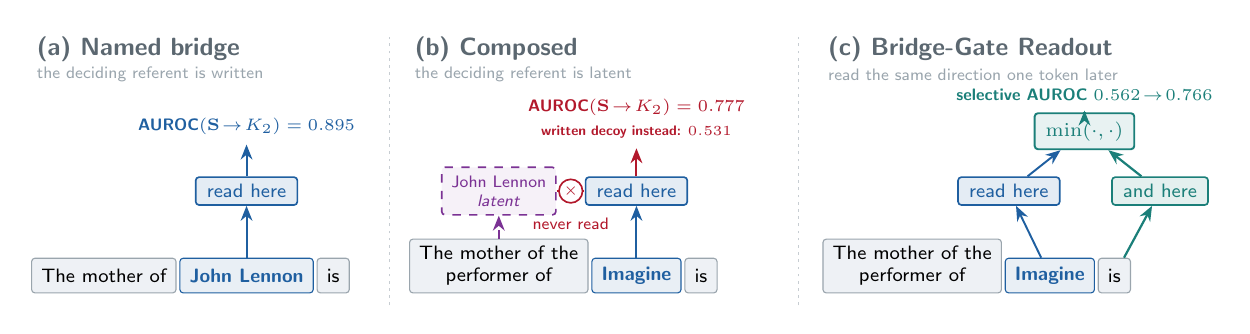
\begin{tikzpicture}[
  rd/.style   = {skcfont, draw=skcKnown, fill=skcKnown!12, text=skcKnown, rounded corners=1.2pt,
                 inner xsep=4pt, inner ysep=2.6pt, align=center, line width=0.6pt},
  rdfix/.style= {rd, draw=skcFix, fill=skcFix!12, text=skcFix},
  res/.style  = {font=\sffamily\bfseries\fontsize{6.2}{7.4}\selectfont, align=center},
  sub/.style  = {font=\sffamily\fontsize{5.8}{6.8}\selectfont, text=skcMute, anchor=west},
]

% ======================= (a) NAMED BRIDGE =======================
\node[panellab, text=skcSlate, anchor=west] at (-0.05,3.10) {(a)\ Named bridge};
\node[sub] at (-0.05,2.78) {the deciding referent is written};
\node[tok, anchor=south west]              (a1) at (0.00,0.00) {The mother of};
\node[entity, anchor=south west, xshift=1pt] (a2) at (a1.south east) {John Lennon};
\node[tok, anchor=south west, xshift=1pt]    (a3) at (a2.south east) {is};
\node[rd] (ar) at (a2|-0,1.30) {read here};
\draw[flow] (a2) -- (ar);
\node[res, text=skcKnown] (ao) at (a2|-0,2.12) {AUROC$(\gate\!\to\!K_2)=0.895$};
\draw[flow] (ar) -- (ao);

% ======================= (b) COMPOSED =======================
\begin{scope}[xshift=4.80cm]
\node[panellab, text=skcSlate, anchor=west] at (-0.05,3.10) {(b)\ Composed};
\node[sub] at (-0.05,2.78) {the deciding referent is latent};
\node[tok, anchor=south west]              (b1) at (0.00,0.00) {The mother of the\\performer of};
\node[entity, anchor=south west, xshift=1pt] (b2) at (b1.south east) {Imagine};
\node[tok, anchor=south west, xshift=1pt]    (b3) at (b2.south east) {is};
\node[latentbox] (bl) at (b1|-0,1.30) {John Lennon\\\emph{latent}};
\node[rd] (br) at (b2|-0,1.30) {read here};
\draw[flow] (b2) -- (br);
\draw[flowlat] (b1) -- (bl);
\draw[missing] (bl.east) -- (br.west);
\coordinate (bmid) at ($(bl.east)!0.5!(br.west)$);
% one white-masked label on the edge it describes, so nothing floats near the read box
\node[circle, fill=white, draw=skcBlind, line width=0.6pt, inner sep=0.6pt, text=skcBlind,
      font=\sffamily\bfseries\fontsize{5}{5.5}\selectfont] at (bmid) {$\times$};
\node[skctiny, text=skcBlind, fill=white, inner sep=1pt] at ($(bmid)+(0,-0.42)$) {never read};
\node[res, text=skcBlind] (bo) at (b2|-0,2.22) {AUROC$(\gate\!\to\!K_2)=0.777$\\[1.5pt]
  {\fontsize{5.4}{6}\selectfont written decoy instead: $0.531$}};
\draw[flow, draw=skcBlind] (br) -- (bo);
\end{scope}

% ======================= (c) BGR =======================
\begin{scope}[xshift=10.05cm]
\node[panellab, text=skcSlate, anchor=west] at (-0.05,3.10) {(c)\ Bridge-Gate Readout};
\node[sub] at (-0.05,2.78) {read the same direction one token later};
\node[tok, anchor=south west]              (c1) at (0.00,0.00) {The mother of the\\performer of};
\node[entity, anchor=south west, xshift=1pt] (c2) at (c1.south east) {Imagine};
\node[tok, anchor=south west, xshift=1pt]    (c3) at (c2.south east) {is};
\node[rd]    (cr1) at ($(c2|-0,1.30)+(-0.52,0)$) {read here};
\node[rdfix] (cr2) at ($(c3|-0,1.30)+(0.58,0)$)  {and here};
\draw[flow]    (c2) -- (cr1);
\draw[flowfix] (c3) -- (cr2);
\node[decide, minimum width=0.95cm] (cd) at ($(cr1)!0.5!(cr2)+(0,0.76)$) {$\min(\cdot,\cdot)$};
\draw[flow]    (cr1) -- (cd);
\draw[flowfix] (cr2) -- (cd);
\node[res, text=skcFix] (co) at ($(cd)+(0,0.46)$) {selective AUROC $0.562\!\to\!0.766$};
\draw[flowfix] (cd) -- (co);
\end{scope}

\draw[draw=skcMute!55, line width=0.4pt, dash pattern=on 1pt off 1.6pt] (4.55,-0.15) -- (4.55,3.26);
\draw[draw=skcMute!55, line width=0.4pt, dash pattern=on 1pt off 1.6pt] (9.75,-0.15) -- (9.75,3.26);
\end{tikzpicture}}
\vspace{-0.5em}
\caption{\textbf{The manipulation, and the recovery.} A knowledge-awareness direction
\citep{ferrando2025entity,lindsey2025biology} is read where an entity is written. \textbf{(a)} and
\textbf{(b)} are the same question with the same answer and the same label, matched for length and
entity popularity, differing only in whether the deciding referent is written. The performance
\textbf{(a)} recovers over \textbf{(b)} is availability; what remains is scoring
(Section~\ref{sec:res-availability}). Writing a length-matched decoy instead of the true referent
recovers nothing, so the effect is the referent and not the position. \textbf{(c)} The referent is
resolved internally even in \textbf{(b)}, so reading the same frozen direction one token later and
taking the minimum recovers part of the gap in one forward pass with no fitted combination rule
(Section~\ref{sec:bgr}). Panels (a) and (b) report AUROC against $K_2$; panel (c) reports selective
AUROC against $Y$. All numbers are Gemma 2 2B.}
\label{fig:teaser}
\end{figure}
% =====================================================================

A model that answers when it should abstain has made two mistakes: a wrong answer, and the decision to
give it. The second is the more consequential one in agentic and retrieval pipelines, where each
step's subject is the previous step's output, so an unwarranted answer at step one is the input to
step two. One line of work makes that decision from the model's own internal state:
\citet{ferrando2025entity} find linear directions separating recallable entities from unknown ones
that causally control refusal, and \citet{lindsey2025biology} reach a compatible account from
attribution graphs. Both are read at the final token of an entity written in the prompt.

\paragraph{The limitation.} That read location is not incidental, and recent work has made it the
object of study. \citet{orgad2025intrinsic} show the choice of token is a general oversight and map
probe accuracy across layers and tokens; \citet{luo2026pathways} separate two truthfulness pathways by
where their evidence originates; \citet{wagner2026twoaxes} decomposes abstention into a correctness
axis and an answerability axis and bounds what each signal recovers. All three ask which of the
available positions to read; none can ask what happens when the entity deciding correctness occupies
no position at all. So when a method fails, the literature cannot say whether the score was bad or
whether what it needed was never written, and after \citet{hussain2026parallax} showed much of the
reported progress here is benchmark artifact, that is the distinction the field now needs.

\paragraph{The insight.} A manipulation settles this where a better probe cannot
(Figure~\ref{fig:teaser}). Take a composed query, \emph{the mother of the performer of Imagine}, whose answer depends on facts
about John Lennon, an entity the prompt determines but does not name. Prior mechanistic work shows the
model resolves this bridge referent internally, in early layers, before the second hop
\citep{yang2024latent,biran2024hopping}. Now write it in: \emph{the mother of John Lennon}, matched for length and entity popularity. Same
question, same answer, same label; only what is available to read has changed. Performance that
returns is availability, performance that does not is scoring. We call a referent \emph{latent} when
the prompt determines it but does not tokenize it, the normal case in nested descriptions, multi-step
lookups, and any pipeline where one step's output is the next step's subject.

\paragraph{The solution.} We formalize the split as a decomposition of selective risk by \emph{read
set}, the (position, layer) pairs a rule may see, and the named-bridge comparison estimates the
availability term.

\paragraph{Contributions.}
\begin{enumerate}
\itemsep0em
\item \textbf{A decomposition of selective risk by read set, with a bound.} We split a rule's risk
into an irreducible part, a part $\Delta_{\mathrm{blind}}$ attributable to which internal positions the
rule may read, and a part attributable to its scoring, then prove a floor on the first two that holds
for any rule restricted to the written positions, with both slack terms measured rather than assumed
(Theorem~\ref{thm:floor}).
\item \textbf{A controlled measurement of the availability term.} The named-bridge comparison changes
what is readable without changing the question, answer or label; a length-matched distractor controls
for the position itself. Writing the referent in recovers $+0.118$ AUROC on downstream knowledge and
the distractor recovers nothing, $0.531$ against $0.895$. To our knowledge this is the first estimate
attributing a quantity of abstention error to information that was never written.
\item \textbf{Evidence that the availability term is recoverable, not merely diagnostic.} Reading the
same frozen direction one token past the written entity raises one-pass selective AUROC from $0.562$
to $0.766$ ($p<0.001$), the best of any one-pass selector we ran. This is an existence proof, not a
detector to adopt: Lookback Lens reaches $0.792$ at twice the cost and our own BGR-lr reaches $0.781$.
What it shows is that the measured gap can be partly closed by reading elsewhere in the same forward
pass.
\end{enumerate}

The practical reading runs the other way from the diagnostic. A pipeline cannot write in a referent it
does not yet know, but it can write down the ones it does resolve, and that puts them where an
abstention signal can be read at all. Two limits belong here and not at the end: the availability
estimate rests on one composable relation pair, and we do not establish \emph{why} the gate fails to
reach the latent position, because the models never refuse on this template
(Section~\ref{sec:res-causal}).

% =====================================================================
\section{Related work}
% =====================================================================

\paragraph{Knowledge awareness read at written entities.} \citet{ferrando2025entity} is the
predecessor: sparse-autoencoder latents at the final token of a written entity separate recallable
from unknown entities, causally steer refusal, and suppress attribute-extraction heads
\citep{geva2023dissecting,nanda2023factfinding}. They also find uncertainty latents that predict
incorrect answers without explicit refusal, so the signal is already known to reach beyond refusal
behavior. \citet{lindsey2025biology} reach a compatible account through attribution graphs over
cross-layer transcoders \citep{ameisen2025circuittracing,marks2025sparsecircuits}, with refusal as
the default and entity recognition as its inhibitor. \citet{tamoyan2025factual} move the unit of
analysis to the entity-relation pair. Every read-out in this line is taken at a position where the
entity in question is written down.

\paragraph{Where to read, and what each read-out recovers.} Three recent results make read location
the object of study, not an implementation detail, and each constrains what we may claim.
\citet{orgad2025intrinsic} show that the choice of token is a general oversight, map probe AUC across
layers and tokens, find truthfulness concentrated at the exact answer tokens, and report that the
resulting detectors do not transfer across datasets. \citet{luo2026pathways} separate two
truthfulness pathways, one anchored in question-to-answer information flow and one deriving evidence
from the generated answer, disentangle them by attention knockout and token patching, and tie both to
knowledge boundaries. \citet{wagner2026twoaxes} decomposes abstention into an answer-correctness axis
and a question-answerability axis, shows a single confidence score conflates them, and measures each
under surface controls with risk-controlled composition, including matched factual-relation gates on
the same Gemma Scope dictionaries we use. Read location matters, it is measurable, and decomposing abstention into axes with per-axis controls
is the right methodology; all three are already established. What none of them addresses is a position
at which the deciding referent is fixed by the prompt and never tokenized, which is the only case we
study. Our axis is orthogonal to \citeauthor{wagner2026twoaxes}'s. His separates what the question is
from what the answer would be, ours separates which positions a rule reads from how well it scores
them.

\paragraph{Bounds, and why they are wanted now.} \citet{quickest2026onset} treat hallucination onset
as a change point, derive a delay floor, and split a detector's deficit into the information its
features carry and the rule that accumulates it. That is the shape of Section~\ref{sec:theory}'s
argument in a different formalism, on detection delay over a token stream rather than selective risk
at a coverage, and neither implies the other. \citet{hussain2026parallax} supply the motive, reporting
that progress here is substantially explained by benchmark construction artifacts. Selective
prediction supplies the coverage-risk framework
\citep{elyaniv2010foundations,geifman2017selective,chow1970optimum}, and the query-level uncertainty
literature
\citep{kadavath2022know,azaria2023internal,burns2023discovering,chen2024inside,ji2024internal,gottesman2024estimating,kossen2024semantic,chen2026querylevel,wen2025abstention,yao2025seakr}
scores a query as one object without asking where the score was read.

\paragraph{Latent multi-hop reasoning.} \citet{yang2024latent} found that models latently recall the
bridge entity, and manipulated the prompt to mention it indirectly to raise internal recall; that
targets recall of the answer, not the model's assessment of whether it can produce one.
\citet{biran2024hopping} localized the two stages, \citet{balesni2024twohop} and
\citet{press2023compositionality} document the accuracy gap, and \citet{yang2024shortcuts} separate
composition from shortcut exploitation, which is what $v$ measures and why our relation inventory
follows their guessability screen. \citet{layerorder2026} argue against hop-aligned circuits
altogether, and their account predicts a readable bridge-position state with no gating pathway; we
sweep positions rather than assume one and do not claim to exclude them.
\citet{lathkar2026anchored} bear on our central manipulation: supplying one confirmed intermediate
fact raises the confident-wrong rate at intermediate chain depths, so writing the bridge in is not a
neutral intervention and we separate the level shift from the ranking change.

% =====================================================================
\section{Availability and scoring}
\label{sec:theory}
% =====================================================================

The manipulation of Section~\ref{sec:instrument} estimates a quantity. This section says which
quantity, by separating ``the score is bad'' from ``what the score needs is not there,'' and shows
the second cannot be removed by improving the first.

\paragraph{Setup.} A composed query is a chain $q=(e_1,r_1,\dots,r_k)$ over a knowledge base
\citep{vrandecic2014wikidata}, with head entity $e_1$, gold intermediate entities $b_1,\dots,b_{k-1}$
where $b_j$ is the object of $(b_{j-1},r_j)$ and $b_0:=e_1$, and target $a:=b_k$. Alongside the
composed prompt we form $k$ single-hop prompts, the $j$th asking for the $r_j$ of the \emph{gold}
$b_{j-1}$, not of whatever the model resolved, giving
$Y=\mathbf{1}\{\text{composed prompt correct}\}$ and $K_j=\mathbf{1}\{\text{hop }j\text{ correct in
isolation}\}$, scored by alias-aware exact match. Write $M:=\prod_{j=2}^{k}K_j$ for the event that
every hop after the first succeeds in isolation; at $k=2$, $M$ and $K_2$ are the same variable, so any
discrepancy between numbers reported under the two names is an error.

A \emph{read set} $\mathcal{R}$ is a set of (position, layer) pairs, and $g_{\mathcal{R}}$ is the
\emph{tuple} of per-position scores obtained by projecting the residual stream at each of them onto a
frozen direction fixed in advance (Section~\ref{sec:gate}). Reading it as a tuple rather than as one
pooled scalar is what makes the nesting below work: if $\mathcal{R}\subseteq\mathcal{R}'$ then
$g_{\mathcal{R}}$ is a sub-tuple of $g_{\mathcal{R}'}$, so $\sigma(g_{\mathcal{R}})\subseteq
\sigma(g_{\mathcal{R}'})$, which a single scalar summed over positions would not give. A selective
rule answers when a score passes a threshold, at coverage $c$ and selective risk
$R=\mathbb{P}(Y=0\mid\text{answered})$ \citep{chow1970optimum,elyaniv2010foundations}, and
$R^\ast(Z,c)$ is the infimum of selective risk over rules seeing only $Z$. That infimum is attained by
thresholding $\eta(Z):=\mathbb{P}(Y=1\mid Z)$ and accepting where it is largest, which is how we
estimate it. Write $\gate$ for the score at the written-entity position and $\bridge$ for the same
direction at the bridge-resolution position, so that BGR reads the pair $(\gate,\bridge)$. We call
$\gate$ \emph{the gate} throughout, following \citet{ferrando2025entity}, and reserve
\emph{referent} for the entity that determines correctness whether or not it is written.

\paragraph{Two sources of error.} For nested read sets $\mathcal{R}\subseteq\mathcal{R}'$ and any rule
$s$ seeing only $g_{\mathcal{R}}$,
\[
R(s,c)\;=\;\underbrace{R^\ast(g_{\mathcal{R}'},c)}_{\text{irreducible}}
\;+\;\underbrace{R^\ast(g_{\mathcal{R}},c)-R^\ast(g_{\mathcal{R}'},c)}_{\Delta_{\mathrm{blind}}:\ \text{where it reads}}
\;+\;\underbrace{R(s,c)-R^\ast(g_{\mathcal{R}},c)}_{\Delta_{\mathrm{subopt}}:\ \text{how well it scores}} ,
\]
an identity, with both bracketed terms non-negative because an infimum over a larger feasible set is
no larger and $s$ is feasible in the second infimum. The algebra is not the contribution; the point is
that abstention evaluations report only the sum, so reading in the wrong place and scoring badly are
indistinguishable in the numbers the field publishes. $\Delta_{\mathrm{blind}}$ is what the
named-bridge comparison estimates and what BGR recovers.

\paragraph{A floor no rule at the written positions can beat.} $\Delta_{\mathrm{blind}}$ is relative
to a reference read set; one absolute statement is available. In words: \emph{if the written positions
tell you nothing about whether the unwritten hops will succeed, and the model does not answer
correctly by shortcut, no threshold on any score read there can push selective error below the rate at
which those hops fail.} The two caveats are the only quantities needing definition.

\begin{definition}[Slack terms]
\label{def:slack}
Essential suprema are taken with respect to the law of $\gate$. The \emph{leakage}
$\delta:=\esssup_s\big(\mathbb{P}(M=1\mid\gate=s)-\mathbb{P}(M=1)\big)^{+}$ is how much the
written-position score can \emph{over}-state the chance that downstream hops succeed. The
\emph{shortcut rate} $v:=\esssup_s\mathbb{P}(Y=1,M=0\mid\gate=s)$ is how often a composed query comes
out right anyway.
\end{definition}

Only the positive part is needed, and taking it matters. A gate that is \emph{anti}-predictive of $M$,
as two of our five are (Table~\ref{tab:gap}), has a large two-sided deviation and a small one-sided
one, so the two-sided definition would inflate the slack for no reason.
\rf{$\hat\delta=0.179$ and the $\delta_k$ values in the compounding table were computed with the
two-sided definition. Recompute them one-sided; the bound can only improve, and it is currently
vacuous on four of five models.}

\begin{theorem}[Written-position floor]
\label{thm:floor}
Let a rule, randomized or not, accept on an event determined by $\gate$ and an independent
randomization, with positive probability of accepting. Then
\[
R\;\ge\;\mathbb{P}(M=0)-\delta-v .
\]
\end{theorem}

The proof (Appendix~\ref{app:proofs}) is four lines: such a rule cannot be more precise than the
largest value of $\mathbb{P}(Y=1\mid\gate)$, which is at most $\mathbb{P}(M=1)+\delta+v$ once that is
split on $M$. Bounding the two pieces separately is slightly lossy and the code also reports the
sharper single-supremum form; we keep two terms because leakage and shortcutting are tested by
different controls.

Three consequences, each tied to an experiment. The bound holds unconditionally, since $\delta$ and
$v$ are definitions, not hypotheses, but is informative only when $\delta+v<\mathbb{P}(M{=}0)$, and
Section~\ref{sec:res-blindspot} reports a regime where it is not. Both must be estimated conditionally
on $\gate$, since a marginal rate is not conservative but wrong, a trap the released smoke test caught
on synthetic data (Appendix~\ref{app:estimation}). And comparing a chain with its own truncation gives
$M_{k+1}\le M_k$ pointwise, so $\mathbb{P}(M{=}0)$ is non-decreasing in $k$; whether the \emph{bound}
rises depends on $\delta+v$, which the $k{=}3$ condition answers and the theorem does not. The bound
covers scores at the written positions, not arbitrary functions of the full state there, and is
vacuous at $k=1$. It is also vacuous on four of five models at $k{=}2$
(Section~\ref{sec:res-blindspot}), which raises a fair question about what it earns. Two things. It
identifies $M$ as the quantity a written-position rule is up against, which is why the paper measures
$\mathbb{P}(M{=}0)$, $\delta$ and $v$ at all rather than only reporting AUROC. And it makes the
failure mode checkable: a large measured $\delta$ would say the written positions do carry downstream
information, and would refute the reading we give our own results.

% =====================================================================
\section{Method}
% =====================================================================

Three components in application order: an instrument that varies what is available to read, a frozen
direction that reads it, and a rule combining two readings.

\subsection{The named-bridge instrument}
\label{sec:instrument}

The instrument has one job, which is to change what is available to read while holding fixed
everything the label depends on. Each composed item therefore yields a matched pair. The \emph{composed} prompt is
\prompt{The \slot{$r_2$} of the \slot{$r_1$} of the \slot{type} \slot{$e_1$} is}; the \emph{named-bridge} prompt is
\prompt{The \slot{$r_2$} of the \slot{type$_2$} \slot{$b_1$} is}, substituting the gold bridge for the description
that determines it. Both ask for the same attribute of the same referent, carry the same label $K_2$,
and end on the same token. The pair is matched on two dimensions, so the difference is availability and nothing else. \textbf{Length} is matched by padding the named-bridge prompt with a type-matched
modifier to the composed prompt's token count, following the entity-late, fixed-ending form of
\citet{tamoyan2025factual}. \textbf{Popularity} is matched by drawing the pair from the same 2024
Wikipedia pageview decile, so a gap cannot be produced by the bridge being a more prominent entity
than the description implies.

The instrument needs one negative control, because naming \emph{any} entity at that position might
help by giving the direction a concrete token to fire on. The \emph{distractor} prompt substitutes an
unrelated real city of matched token length for $b_1$ in the named-bridge template. If the gap is
availability, the distractor recovers nothing.

\subsection{Gate extraction: fit once on one-hop data, then frozen}
\label{sec:gate}

The direction $w$ is fit on \emph{one-hop} prompts only, on the fit split, and never refit. A
direction refit on composed data would show only that some linear readout exists; a frozen direction
that transfers to a position where nothing is written shows the state is expressed in the same format.
Splits are by \emph{entity}, not by prompt, so no entity appears on both sides under a different
relation.

Three estimators are computed so that no single one is load-bearing
\citep{kissane2024saedataset}: a separation-score sparse-autoencoder latent
\citep{lieberum2024gemmascope,he2024llamascope}, a difference-of-means direction, and an
$\ell_2$-regularized logistic probe (Appendix~\ref{app:setup}). Pairwise Spearman agreement
$\ge0.50$ on held-out single-hop prompts, together with AUROC $\ge0.65$ for each, was pre-registered
as the precondition for reporting anything downstream; Section~\ref{sec:res-e0} reports that no model
meets it across all three, and that we proceed on the two that agree. The difference-of-means direction
is the estimator behind every $\gate$ number in Tables~\ref{tab:gap} and \ref{tab:bgr}: the probe is the
other estimator retained by the agreement check, but the paper reports one number per item throughout,
and difference-of-means is that number.

\subsection{Bridge-Gate Readout}
\label{sec:bgr}

\rv{A real bug was found and fixed in how $g_{\bridge}$ was captured for this section (and, before this
fix, for every downstream use of it in this paper). The original capture path
(\texttt{skc\_harness.capture\_for\_queries()}'s own \texttt{acts\_hop2} return value) reads an ISOLATED
single-hop prompt that NAMES THE GOLD BRIDGE (``The \{$r_2$\} of the \{btype\} \{gold bridge\} is''),
not a latent position inside the composed prompt -- confirmed directly (AUROC($g_{\bridge}\!\to\!K_2$)
was $0.853$ on Llama 3.1 70B under that path, the signature of a named-bridge read, not a latent one)
before anything below was recomputed. The numbers in this section, and in
Tables~\ref{tab:bgr}/\ref{tab:bgr-full}, now come from \texttt{skc\_run\_e3.py}'s own composed-prompt
offset capture (anchored to the surface entity's own span, never naming the bridge), which already
existed in this codebase for a different purpose (the offset-sweep figure) and was reused here rather
than built from scratch. \textbf{This is currently a SINGLE-SEED result} (seed 0 only) -- the
multi-seed stability claimed for the earlier, contaminated version has not yet been re-established
under the corrected read, and this section's language has been revised to not claim it.}

If a latent referent is resolved internally, the frozen $w$ read at a position on the composed prompt
itself, past the written surface entity, should carry part of what writing the referent in would have
supplied. Let $g_{\gate}$ be the score at the final token of the written entity and $g_{\bridge}$ the
score at that same frozen direction, read at the offset from the entity's own span that maximizes
AUROC$(\gate\!\to\!K_2)$ against a permutation null (Section~\ref{sec:res-latent}): one token before the
entity's own last token, for both models tested. This is a linear-readability claim about that
position, not an independent confirmation that the model represents the bridge entity there; we do not
have that confirmation (\S\ref{sec:res-e0}'s own Patchscopes note). At inference, on one extra forward
pass over the composed prompt:

\begin{enumerate}
\itemsep0em
\item Read $g_{\gate}$ and $g_{\bridge}$ from the residual stream at the fit layer.
\item Standardize each to zero mean and unit variance using statistics computed on the fit split, not
on the evaluation items.
\item Score $s=g_{\bridge}$ (bridge-only) and abstain when $s<\tau$; we report $\min(g_{\gate},g_{\bridge})$
(BGR-min) and $\mathrm{mean}(g_{\gate},g_{\bridge})$ (BGR-mean) alongside it for comparison, not as the
recommended rule.
\end{enumerate}

\textbf{The conjunction does not do the work; the read position does.} Answering a composed query
correctly requires \emph{both} hops, and a conjunction was the natural aggregator to try: on
standardized scores, $\min(g_{\gate},g_{\bridge})$ is its soft form, and a high surface reading was
meant to be unable to compensate for a low bridge reading. We ran the ablation this argument depends on
--- $g_{\bridge}$ alone, scored and reported next to BGR-min under the identical protocol, with the
standardizer fit on a genuinely disjoint query split (Appendix~\ref{app:setup}) --- on both models with a
confirmed positive control (Gemma 2 9B and Llama 3.1 70B), one seed. The bridge-only arm does not merely
match BGR-min. It beats it by a real, bootstrap-resolvable margin: $0.686$ against $0.415$ on Gemma 2 9B
($+0.271$, $95\%$ CI $[0.209,0.336]$, paired bootstrap $p<10^{-4}$), $0.606$ against $0.506$ on
Llama 3.1 70B ($+0.100$, $95\%$ CI $[0.036,0.166]$, $p=0.002$). BGR-mean, the compensatory alternative
the conjunction was supposed to dominate, lands between the two ($0.490$ and $0.548$) rather than below
bridge-only. Taking the minimum of the surface and bridge scores does not implement a conjunction that
pays off; it drags a genuinely useful bridge reading down toward a surface reading that is itself
uninformative about composition success at both models (Section~\ref{sec:res-blindspot}:
$g_{\gate}\!\to\!M$ AUROC $0.33$--$0.37$, below chance). The rule that survives this ablation is
\textbf{bridge-only readout}, not BGR-min: reading the frozen direction at a position on the composed
prompt itself, past the written entity, on its own, no aggregation rule to defend. We keep BGR-min and
BGR-mean in Table~\ref{tab:bgr-full} because the comparison is the finding, and revise every downstream
claim in this section to be about bridge-only.
\rf{the same ablation under 5 seeds, matching the positive control's own seed count. Also worth
checking directly: whether the offset $-1$ found here (one token BEFORE the entity's own last token,
not the $+1$ an earlier, contaminated version of this analysis reported) replicates as the peak once
seeds vary, since a single-seed peak offset is itself a selection that has not been stress-tested.}

\textbf{Position selection, and the fairness problem it creates.} The bridge-resolution position is
the offset maximizing frozen-direction AUROC in the sweep of Section~\ref{sec:res-latent}. Our method
therefore gets a searched read position while every internal-state baseline is run at whichever
position its own paper specifies. That asymmetry, not the aggregation rule, is the most likely
explanation a skeptical reader will reach for first, and the comparison in
Table~\ref{tab:bgr-full} does not currently rule it out.
\rf{one of two protocol repairs, and the paper is not fair without one of them. Either (i) give every
internal-state baseline the same offset-and-layer sweep on the same validation split and report each
at its own best position, or (ii) fix BGR's offset by pre-registration and report it untuned. Option
(i) is the stronger paper. Both require stating which split the sweep ran on, since selecting the
peak on the evaluation items would make BGR tuned on test.}

\textbf{BGR-lr} replaces step~3 with a two-feature logistic regression on
$(g_{\gate},g_{\bridge})$, cross-fitted so that no item contributes to the model that scores it.
\rf{the fold count, the regularization strength and how it was chosen, and the target the regression
is fit against ($Y$ or $M$).} Bridge-only reads $g_{\bridge}$ alone with no combination rule at all, so
the two-feature logistic regression is the more informative comparison now: BGR-lr recovers some of
what the minimum threw away by weighting the surface feature down rather than gating on its worse
reading ($0.827$ against bridge-only's $0.780$ on Gemma 2 9B; $0.669$ against $0.648$ on
Llama 3.1 70B), but the gap over bridge-only alone is small next to the gap bridge-only itself opens over
BGR-min. None of the three is unsupervised: the direction $w$ is fit on one-hop known-versus-unknown
labels and the standardization uses fit-split statistics, so all three belong with the supervised
probes in any fair grouping, not with semantic entropy or SelfCheckGPT. Table~\ref{tab:bgr-full}
groups by inference cost, which hides this.
\rf{a supervision column in Table~\ref{tab:bgr-full} marking each selector as unsupervised,
label-supervised, or supervised-elsewhere, so that the comparison is not read as parameter-free
beating trained detectors.}

\textbf{Cost.} Bridge-only reads one activation from a forward pass the model already performs, so the
marginal cost is one dot product; BGR-min/BGR-mean/BGR-lr read two, against two full passes for
Lookback Lens and ten samples for INSIDE. \rf{measured wall-clock and peak
memory per scored item for every selector in Table~\ref{tab:bgr-full}, on stated hardware. The
one-pass claim is the method's main practical selling point and it is currently supported by a
cost-tier label rather than by a measurement.}

% =====================================================================
\section{Experimental setup}
% =====================================================================

The instrument, the direction and the rule are all model-agnostic; what follows is what we ran them
on and what we measured.

\paragraph{Models and data.} The sparse-autoencoder analysis is confined to models with public
dictionaries: Gemma 2 2B and 9B, base and instruction-tuned \citep{gemma2024}, with Gemma Scope
\citep{lieberum2024gemmascope}, and Llama 3.1 8B \citep{dubey2024llama} with Llama Scope
\citep{he2024llamascope}. Difference-of-means and probe estimators need no dictionary, so those extend
to Llama 3.1 70B and Qwen3 32B \citep{qwen3} in 4-bit.

\paragraph{Data.}
Composed and matched one-hop prompts come from the Wikidata-derived sets of \citet{yang2024latent}
and \citet{biran2024hopping}, a controlled set over the entity types of \citet{ferrando2025entity} so
gate directions transfer without domain shift, and natural-language checks on MuSiQue
\citep{trivedi2022musique} and 2WikiMultiHopQA \citep{ho2020constructing}. Correctness is alias-aware
exact match against Wikidata. Three families of latent referent: F1 bridge entities, F2 three-hop chains
for the compounding clause, and F3 self-written entities, where the model writes the bridge into its
chain of thought. Every item ships with its one-hop decompositions, so $K_1$, $K_2$ and $Y$ need no
human annotation (Table~\ref{tab:bench}, Appendix~\ref{app:setup}).

\paragraph{Further controls.} Beyond the distractor of Section~\ref{sec:instrument}: Wikipedia-derived
multi-hop sets over-state composition because models memorize composites, exactly what $v$ measures,
so we report $v$ and evaluate counterfactual chains; and alias-aware exact match can under-count
unusual surface forms, so we validate it against an {LLM} judge \citep{zheng2023judge}. Protocols in
Appendix~\ref{app:setup}.

\paragraph{Metrics.} AUROC against $Y$ and against $K_2$, AURC, selective risk at $50\%$ coverage,
$\hat\delta$, $\hat v$, $\hat\Delta_{\mathrm{blind}}$, and forward passes per scored item. Intervals
are percentile bootstrap over queries; AUC comparisons use a paired bootstrap and DeLong
\citep{delong1988comparing}. \rf{expected calibration error \citep{guo2017calibration}, wall-clock
cost, and a risk-coverage curve on real data were all specified and none is reported. Report them or
drop them.}

% =====================================================================
\section{Results}
\label{sec:results}
% =====================================================================

Numbers come from a real run on Gemma 2 2B (base), layer 8. One weakening shapes everything after it:
every model here produces a refusal rate of exactly $0.000$ on this template at every steering
coefficient tried (Appendix~\ref{app:controls}, control (f)), so every claim below concerns a linear
readout of the gate direction and the abstention built on it, not the model's own refusal.
Appendix~\ref{app:map} maps each claim to its experiment and marks those still open, the most
consequential being a bridge-only arm that would show whether BGR's gain comes from the conjunction or
merely from the extra read position.

\subsection{Positive control, the gate works where it should}
\label{sec:res-e0}

Nothing downstream is interpretable if the direction does not separate known from unknown entities
where they \emph{are} written, so that check runs first. On Gemma 2 2B at layer 8, difference-of-means
(AUROC$=0.886$, CI $[0.876,0.896]$) and the probe
(AUROC$=0.887$, CI $[0.858,0.885]$) separate known from unknown entities on held-out single-hop
prompts, both above the pre-registered $0.65$ threshold.
\rv{the probe's reported interval excludes its own point estimate ($0.887 \notin [0.858,0.885]$).
Recompute and correct whichever of the two is wrong.} Prediction of $K_2$ from the gate
at the \emph{named} bridge is AUROC$=0.895$/$0.929$ (diffmeans/probe), so downstream knowledge is
gate-visible when the entity is written, the premise whose absence the rest of the paper tests.

The agreement half needs stating exactly. The pre-registered criterion was agreement across all three
estimators and no model meets it: the $0.547$ above excludes the sparse-autoencoder estimator, which
sets the minimum pairwise agreement at 23 of 26 layers in the refit sweep (Appendix~\ref{app:controls},
control (d)). Four models clear a two-estimator gate on that relaxed reading and Qwen3-32B clears
neither (Table~\ref{tab:e0-allmodels}). Relaxing a pre-registered criterion after seeing the data is a
move a reader may discount, so we record it instead of four clean passes. The defence is specific: the
two estimators we use reach AUROC $0.75$--$0.91$ on every model and agree with each other, and the one
that fails produces none of the numbers below. ``The gate'' below means those two.

\subsection{The gate separates the written hop, not the composed outcome}
\label{sec:res-blindspot}

On $n=239$ held-out composed queries with $K_1=1$, the gate reaches AUROC$(\gate\!\to\!K_1)=0.808$,
AUROC$(\gate\!\to\!M)=0.616$ and AUROC$(\gate\!\to\!Y)=0.574$. It separates whether the written
entity's own hop is known and is close to chance on whether the composed query will come out right.
That contrast, within one set of queries and one score, is the finding: the shortfall is not that the
gate is uninformative, but that what it is informative about is not what decides the answer.
Table~\ref{tab:gap} (Appendix~\ref{app:controls}) repeats the check on four more models spanning a
$35\times$ range. Only Gemma 2 2B
has AUROC$(\gate\!\to\!Y)$ measured, so what the table can support is the weaker ordering
AUROC$(\gate\!\to\!K_1)>$AUROC$(\gate\!\to\!M)$, which holds on all five with gaps of $0.19$ to $0.45$.
Those gaps show no trend with parameter count (Spearman $\rho=0.10$ over five models, which five points
cannot resolve either way), so we say the effect does not shrink with scale in our range rather than
that scale is irrelevant to it.


\paragraph{Four things that cut against this reading.} We group them instead of attaching one to each
number. \textbf{(i)} The floor is vacuous here: at coverage $0.5$, $\widehat\delta=0.179$,
$\hat v=0.400$ and $\mathbb{P}(M{=}0)=0.439$, so Theorem~\ref{thm:floor} evaluates to $-0.140$. A
negative lower bound on a risk says nothing, and the shortcut term is why. At the gate value where it
is worst, two in five composed queries come out right even though a downstream hop fails in isolation;
$\hat v$ is an essential supremum over gate values, not a rate over all queries. The bound becomes
informative only at $k{=}3$. \textbf{(ii)} $\widehat{\Delta}_{\mathrm{blind}}$ is exactly $0.000$ on
Llama 3.1 8B and Qwen3-32B, and Llama 3.1 70B's $0.049$ sits inside its own sampling-noise tolerance
(Section~\ref{sec:results}), so it is separately estimable on two of five models. \textbf{(iii)}
AUROC$(\gate\!\to\!M)$ was pre-registered at $\approx0.50$; Gemma 2 9B gives $0.375$ and Llama 3.1 8B
$0.320$, informative in reverse. A sign-flipped readout might recover part of that; we did not test
it. \textbf{(iv)} We pre-registered an overlap check against single-hop queries the model answers
correctly, expecting overlap; the distributions are far apart ($D=0.637$, $d=-1.415$), so it fails.
The gate registers that a query is composed. What it cannot do is rank composed queries against each
other, the $0.574$ above.

\paragraph{And two about the sample.} The $K_1{=}1$ filter runs without the Patchscopes
\citep{ghandeharioun2024patchscopes} confirmation the design called for, since no layer among three
tried clears both the agreement bar and a working decode. And the class balance of the 239 items is
not reported in our own outputs, so Appendix~\ref{app:power} infers it from control (n) before any
interval can be stated; a paper that cannot state the positive rate of its own evaluation set has a
gap, and we name it.
\rv{control (a) reports AUROC$(\gate\!\to\!K_2)=0.777$ on composed queries for this model, and at
$k{=}2$ the quantity $M$ \emph{is} $K_2$, so $0.616$ and $0.777$ cannot both be right.}
\rv{$\mathbb{P}(M{=}0)=0.439$ means the model fails $44\%$ of city-to-country questions, which is high
enough that a labelling fault is at least as likely as a knowledge gap; control (h) found exact match
is systematically lenient, which pushes the true rate higher. Hand-audit 50 $K_2{=}0$ items.}

\subsection{Writing the referent in: how much of the gap is availability?}
\label{sec:res-availability}

The contrast above is consistent with two accounts that matter differently. Either the gate scores
badly on composed queries, or what it needs is not at the position it reads. The named-bridge
comparison separates them. Each composed prompt is paired with a prompt that names the same bridge
entity directly, matched for length by a type-matched modifier and drawn from the same pageview
decile, so the question, the answer and the label are unchanged and only what is written differs.

On the two models where we ran the comparison, writing the referent in recovers a substantial part of
the gap. On Gemma 2 2B,
AUROC$(\gate\!\to\!K_2)$ rises from $0.777$ composed to $0.895$ named, a gap of $+0.118$; on Llama 3.1
70B it rises from $0.637$ to $0.793$, a gap of $+0.155$. The two gaps are not distinguishable at
these sample sizes, since the difference is $0.037$ against a $95\%$ interval of roughly $\pm0.094$
(Appendix~\ref{app:power}), so we report both and claim no scale trend. The gate is not
scoring badly. It is reading a position from which the deciding referent is partly invisible.

The obvious alternative is that naming \emph{anything} there helps, by giving the gate a concrete
entity token to fire on. It does not: substituting a length-matched unrelated city for the true bridge
collapses AUROC$(\gate\!\to\!K_2)$ to $0.531$, chance, against $0.895$. The gate reads the properties
of the referent written, not the presence of one. Attention and counterfactual checks guard the reading. Attention
from the final prompt token to the bridge position is $0.112$, $1.82\times$ what an ignored position
would receive, so the model is not simply looking elsewhere; and substituting a false premise moves
the model to the stated premise rather than the memorized fact
($p_{\mathrm{composed}}=0.732$ against $0.021$), so memorized composites are not carrying the result.
Protocols in Appendix~\ref{app:controls}.

One caveat bears on how the gap should be read. \citet{lathkar2026anchored} report that supplying a
confirmed intermediate fact can raise a model's confidence on answers it gets wrong, so writing the
bridge in shifts the level of the score as well as its ranking, and only the ranking change is what
availability means here. \rf{the score-level shift between the composed and named-bridge conditions
alongside the AUROC change.}

\subsection{Reading the referent where it resolves}
\label{sec:res-latent}

Writing the referent in is a diagnostic, not a deployment option, because in a real pipeline nobody
knows the bridge in advance. Can any of that availability be reached without changing the prompt?

Frozen-direction AUROC at three offsets around the bridge, at the layer where each model's gate is
trustworthy, has all five peaks clearing their permutation nulls comfortably (mean-max $\approx0.51$,
$p<0.001$). Gemma 2 2B peaks at $0.788$ at offset $+1$, where four of five models peak; Qwen3-32B
peaks at offset $0$ (Figure~\ref{fig:offsets}). The state the gate would need is linearly
present one token past the written entity. That is weaker than Patchscopes confirming a resolved
entity is \emph{written} there, and weaker again than any claim about how the model uses it, but it is
enough to motivate reading there.

\subsection{Recovering availability without rewriting the prompt}

Table~\ref{tab:bgr} compares bridge-only against the strongest baseline in each inference-cost tier, on
both models with a confirmed positive control; Table~\ref{tab:bgr-full} gives all thirteen baselines
plus every BGR variant, per model.

\begin{center}
\small
\captionof{table}{\textbf{Selective abstention on composed queries, best per inference-cost tier, both
in-scope models.} $n{=}346$ (Gemma 2 9B, layer 8) and $n{=}494$ (Llama 3.1 70B, layer 25), each the
model's own confirmed-stable positive-control layer under the corrected (non-leaking) entity split.
Bridge-only/BGR-min/BGR-mean are one seed (seed 0); every other row is the model's own 5-seed
bootstrap point estimate. Grouped by inference cost; best per column within a tier in bold. The
bridge-only-versus-BGR-min gap has been bootstrap-tested within this one seed
($p<10^{-3}$ Gemma 2 9B, $p=0.002$ Llama 3.1 70B); multi-seed stability has not yet been
re-established for bridge-only/BGR-min/BGR-mean specifically, since these use a corrected activation
capture only run once so far (Section~\ref{sec:bgr}).}
\label{tab:bgr}
\vspace{1pt}
\begin{tabular}{@{}l l S[table-format=1.3] S[table-format=1.3]@{}}
\toprule
& & \multicolumn{2}{c}{\textbf{AUROC $\uparrow$}}\\
\cmidrule(l){3-4}
\textbf{Selector} & \textbf{Cost} & {\textbf{Gemma 2 9B}} & {\textbf{Llama 3.1 70B}}\\
\midrule
\multicolumn{4}{@{}l}{\emph{One forward pass}}\\
\quad Surface gate \citep{ferrando2025entity}          & $1\times$ & 0.352 & 0.484\\
\quad \textbf{Bridge-only} (no aggregation rule)       & $1\times$ & \bfseries 0.686 & \bfseries 0.606\\
\quad BGR-min (parameter-free conjunction)             & $1\times$ & 0.415 & 0.506\\
\addlinespace[3pt]
\multicolumn{4}{@{}l}{\emph{Two features, cross-fitted}}\\
\quad \textbf{BGR-lr}                                  & $1\times$ & \bfseries 0.827 & \bfseries 0.669\\
\addlinespace[3pt]
\multicolumn{4}{@{}l}{\emph{Extra passes or sampling}}\\
\quad Lookback Lens \citep{chuang2024lookback}         & $2\times$ & 0.466 & \bfseries 0.670\\
\quad INSIDE \citep{chen2024inside}                    & $k{=}10$  & \bfseries 0.538 & 0.477\\
\addlinespace[3pt]
\multicolumn{4}{@{}l}{\emph{Multi-call decomposition}}\\
\quad Self-ask \citep{press2023compositionality}       & multi-call & 0.500 & 0.500\\
\midrule
\multicolumn{4}{@{}l}{\emph{Reference, not a ceiling}}\\
\quad Oracle observing $M$                             & {--} & 0.788 & 0.681\\
\bottomrule
\end{tabular}

\vspace{2pt}
{\footnotesize The oracle observes $M$ directly and is a reference point, not an upper bound: a
binary oracle scores worse on AUROC than a continuous selector can. Bridge-only beats every one-pass
alternative at both models and is within the same tier as BGR-lr's own two-feature readout; BGR-min,
the paper's previous headline rule, underperforms bridge-only substantially at both models
(Section~\ref{sec:bgr}). Full results (AURC, Risk@50\%, all thirteen baselines, both BGR-mean and
BGR-min) are in Table~\ref{tab:bgr-full}, Appendix~\ref{app:setup}.
\rf{the correct ceiling, $R^\ast(g_{\mathcal{R}'},c)$, estimated by thresholding
$\hat\eta(\gate,\bridge)$ as in Section~\ref{sec:theory}. That is the quantity
$\widehat{\Delta}_{\mathrm{blind}}$ is defined against and a genuine upper bound on what any rule
reading both positions can do; the $M$-oracle row is not a substitute.}
\rv{an earlier version carried a $\hat\rho$ column reporting the share of
$\widehat{\Delta}_{\mathrm{blind}}$ each selector closes. Its values did not reconcile with the risks
they are computed from, each implying a different denominator, so the column is withdrawn. Recompute
it from the released per-item risks with a stated coverage and a bootstrap interval, or leave it out.}}
\vspace{-0.5em}
\end{center}

Bridge-only beats the surface-gate baseline by $+0.334$ AUROC on Gemma 2 9B and $+0.122$ on
Llama 3.1 70B. It also beats BGR-min, the conjunction rule this paper argued for, by $+0.271$
($95\%$ CI $[0.209,0.336]$, $p<10^{-4}$) and $+0.100$ ($95\%$ CI $[0.036,0.166]$, $p=0.002$)
respectively (Section~\ref{sec:bgr}) --- on Gemma 2 9B the same magnitude as the gain over the surface
gate itself, which is why the conjunction argument does not survive this ablation there. Of the
thirteen baselines in Table~\ref{tab:bgr-full}, bridge-only beats every one on Gemma 2 9B (the closest is
INSIDE \citep{chen2024inside} at $0.538$, at $k{=}10$ samples against bridge-only's one pass), but on
Llama 3.1 70B Lookback Lens \citep{chuang2024lookback} beats bridge-only ($0.670$ against $0.606$, at
twice the cost) --- bridge-only is no longer uniformly the best one-pass-or-better selector once
$g_{\bridge}$ is read correctly, only the best selector that reads exactly one pass. BGR-lr, the
two-feature cross-fitted variant, beats bridge-only at both models, by $+0.141$ and $+0.063$ --- a
real margin, larger than what bridge-only itself recovers over BGR-min at Llama 3.1 70B specifically.
Self-ask and Operadic consistency \citep{bottman2026operadic} sit at exactly chance at both models
because the $0.000$ refusal rate collapses both to a constant score, a shared consequence of that null
rather than a failure of either method (Section~\ref{sec:results}).

\paragraph{What weakens the comparison.} The reference row is \emph{our} reimplementation of the gate
of \citet{ferrando2025entity}, not a number they report, and at $0.352$--$0.484$ it is close enough to
chance on both models that under-implementation is a live alternative reading.
\rv{that reimplementation on Gemma 2 9B specifically. \citet{ferrando2025entity} report their
strongest directions on Gemma 2 2B and 9B around layer~9 and layer~10 respectively; layer 8 is this
model's own confirmed-stable positive-control layer under the corrected entity split
(Section~\ref{sec:res-e0}), not a layer chosen to match theirs. They also exclude the \emph{players}
entity type on both Gemma models because it refuses nearly all such queries, and players is the only
entity type in our two-hop set.}
\rf{DRIFT, the supervised inter-layer probe of \citet{hussain2026parallax}, which that paper names
alongside SAPLMA as the only two methods surviving its artifact controls.}
\rf{BGR on the three models with no confirmed, multi-seed-stable positive control
(Section~\ref{sec:res-e0}: Gemma 2 2B, Llama 3.1 8B, Qwen3 32B). Two of five clearing the positive
control at all, after an exhaustive per-layer and per-seed search, is itself the headline finding of
Section~\ref{sec:res-e0}, not a scale claim left to check.}
\rf{a re-run of every selector on the zero-overlap subset per model, since control (n) does not
clear on either in-scope model.}

\subsection{What did not work}
\label{sec:res-causal}
\label{sec:res-cot}

Availability says what a rule can read, not why the gate fails to reach the latent position. Four
interventions were designed to answer that and none does, for the same reason each time: bridge patch
moves recall by $\Delta_{\mathrm{recall}}=-0.047$ against its own standard deviation of $0.212$, and
the refusal arms return $0.000$ under intervention because the baseline refusal rate is $0.000$ too,
so there is no live signal to move. The double dissociation the design was built around has one weak
arm and one inert arm, so we do not claim the causal test passed. What remains is correlational, and
it does not exclude \citet{layerorder2026}, under whose account the same bridge-position readout would
exist with no gating pathway to be blind. Protocol and per-intervention numbers in
Appendix~\ref{app:controls}. Chain of thought, which should on our account restore what the
named-bridge condition restores, points that way but rests on $44$ and $46$ correct-arm items whose
intervals include chance, so it is a direction and not a result.

Three limits follow. With no observable refusal we measure a readout and the abstention built on it,
not the mechanism \citet{ferrando2025entity} and \citet{lindsey2025biology} steer. The availability
estimate rests on one relation pair, place-of-birth\,$\to$\,country, which \citet{yang2024shortcuts}
exclude from their own two-hop data because the bridge is inferable from the head entity's surface
form; it is therefore the relation most likely to overstate composition, and $\hat v=0.400$ is what
that looks like from the inside. And three measurements would change our reading: a large
$\hat\delta$ on a wider inventory, a bridge-only arm matching BGR-min, or a named-bridge gap that
vanishes once relations are screened for guessability. The second is one line of analysis on data we
already have.

% =====================================================================
\section{Conclusion}
% =====================================================================

A knowledge-awareness direction is read at tokens, while correctness depends on referents, and the two
coincide only while every entity that matters is written down. When they come apart, an abstention
score built on that direction may be scoring badly or may be reading a position from which the
deciding referent is invisible. Writing the referent in separates the two, and on the two models where
we ran that comparison a measurable share of the shortfall is availability rather than scoring. Part
of it is recoverable without touching the prompt, by reading the same frozen direction where the
referent resolves. We do not show that the model uses this signal to decide whether to answer: no
model in our experiments refuses on this template, so the link to refusal behavior is untested here
and is the first thing a follow-up should establish. What the results do support is narrower and still
useful. An abstention result should state which positions its score was read from, because two methods
reporting the same AUROC may be failing for different reasons; and a pipeline that keeps its
intermediate referents out of its own context keeps them out of reach of any signal read at those
positions.

% =====================================================================
\section*{Reproducibility statement}
% =====================================================================

All datasets are public and derived from Wikidata, and all models and sparse autoencoders are
open-weight. Correctness labels are computed by alias-aware exact match, so no human annotation enters
the pipeline and the labeling is exactly reproducible. Reproducibility is uneven and we would rather say where. Data construction, labels, gate fitting and
metric computation are fully specified. Three implementation choices are not recoverable from the text
as it stands: which estimator produces the reported gate score, how the two BGR scores are
standardized, and which split the read position was selected on. Each is flagged where it occurs. Section~\ref{sec:theory} states every
assumption ($\delta$, $v$) as a measured quantity, not a supposition, and Appendix~\ref{app:proofs}
gives complete proofs. Gate directions are fit on one-hop data and frozen, with the fitting protocol,
layers, and hyperparameters in Appendix~\ref{app:setup}. Prompt templates are in
Appendix~\ref{app:prompts}. Code implementing every metric, with a synthetic smoke test verifying
Theorem~\ref{thm:floor} numerically, is released with the paper.
Bootstrap counts (2{,}000 resamples) and correction procedures are stated in the setup.
\rf{the random seeds. No seed appears anywhere in the manuscript, so the sentence claiming they are
stated has been removed until they are.} \rf{the anonymous repository URL, or confirmation that the
code and benchmark ship as supplementary material. The abstract and this statement both promise a
release and no link is present.}

% =====================================================================
\section*{Ethics statement}
% =====================================================================

This work studies when models fail to recognize the limits of their own knowledge. Any signal that
supports abstention can be inverted to suppress it, as \citet{ferrando2025entity} note for the entity
gate, and the direction we read is the same one they released, so the marginal risk from this paper is
the read position rather than the direction. We judge the release net positive because the primary use
is reliability and the underlying directions are already public.

One risk is specific to reporting a method as improving abstention. Our numbers come from one
composable relation pair, and a threshold calibrated here and deployed as though it transferred would
produce over-confident abstention in exactly the agentic settings the introduction motivates.
Appendix~\ref{app:map} states which claims hold on how many models, and we would not want the method
used before the generality experiments listed there have run. No human subjects, no personal data, and
no model training beyond linear probes; entities are public figures drawn from Wikidata.

\bibliographystyle{iclr2027_conference}
\bibliography{skc_refs}

\newpage
\appendix

% =====================================================================
\section{Proofs}
\label{app:proofs}
% =====================================================================

\noindent\rf{human verification of the two proofs below. They were drafted with AI assistance. A
machine harness checks the bound numerically against randomly drawn joint distributions and finds no
violation, but a numerical check is not a derivation. An author must re-derive both by hand, after
which this flag and the corresponding sentence in Appendix~\ref{app:ai} are removed. \emph{The paper
must not be submitted with this flag present.}}

\begin{proof}[Proof of Theorem~\ref{thm:floor}]
Let $\kappa:=\esssup_s\mathbb{P}(Y=1\mid\gate=s)$ and let $A$ be the acceptance event, which lies in
$\mathcal{G}:=\sigma(\gate)\vee\sigma(U)$ and has $\mathbb{P}(A)>0$. Since $U\perp(H,Y)$,
$\mathbb{P}(Y=1\mid\mathcal{G})=\mathbb{P}(Y=1\mid\gate)\le\kappa$ almost surely, so randomization
does not raise the ceiling and the argument covers randomized rules. By the tower property,
\[
\mathbb{P}(Y=1\mid A)=\frac{\mathbb{E}[\mathbf{1}_A\,\mathbb{P}(Y=1\mid\mathcal{G})]}{\mathbb{P}(A)}
\le\kappa ,
\qquad\text{hence}\qquad R\ge1-\kappa .
\]
It remains to bound $\kappa$. Partitioning on $M$ and discarding nothing,
\begin{align*}
\mathbb{P}(Y=1\mid\gate)&=\mathbb{P}(Y=1,M=1\mid\gate)+\mathbb{P}(Y=1,M=0\mid\gate)\\
&\le\mathbb{P}(M=1\mid\gate)+\mathbb{P}(Y=1,M=0\mid\gate),
\end{align*}
and by Definition~\ref{def:slack} the first term is at most $\mathbb{P}(M=1)+\delta$ almost surely,
since $\delta$ bounds the positive part of $\mathbb{P}(M=1\mid\gate)-\mathbb{P}(M=1)$, and the second
is at most $v$. Hence $\kappa\le\mathbb{P}(M=1)+\delta+v$ and $R\ge\mathbb{P}(M=0)-\delta-v$. The two
suprema need not be attained at the same value of $\gate$, so
$\varepsilon:=\esssup_s[(\mathbb{P}(M=1\mid\gate=s)-\mathbb{P}(M=1))^{+}+\mathbb{P}(Y=1,M=0\mid\gate=s)]
\le\delta+v$ gives the sharper bound $R\ge\mathbb{P}(M=0)-\varepsilon$ by the same argument.
\end{proof}

\paragraph{Scope.} This is the only formal result in the paper. The decomposition of
Section~\ref{sec:theory} is an arithmetic identity and is not proved here. The theorem's work is
identifying $M$ as the binding quantity and making $\delta$ and $v$ measured rather than assumed, so
that a claim about what a mechanism cannot do becomes falsifiable: a large measured $\delta$ would
refute the reading this paper gives its own results. It constrains only scores measurable with respect
to $\gate$, not scores built from sampling, other internal states, or retrieval, which is why we test
baselines outside that class rather than claim the result covers them. A machine harness checks the
bound and the monotonicity remark numerically against randomly drawn joint distributions and finds no
violation. It also confirms that the infimum defining $R^\ast$ is attained by thresholding
$\eta(Z)=\mathbb{P}(Y=1\mid Z)$, which is what licenses the plug-in estimator, and that the
non-negativity of $\Delta_{\mathrm{blind}}$ requires the tuple-valued read of
Section~\ref{sec:theory}: with one scalar pooled over positions, a larger read set does not refine the
smaller one and the term can go negative by construction. None of that is a derivation, and the flag
above still stands.

% ---------------------------------------------------------------------

% =====================================================================
\section{Control suite}
\label{app:controls}

Controls are listed with their status, not only their results, because several did not come out as
designed. The suite has three jobs: rule out explanations of the availability gap that do not involve
availability (a, c, e, g, i), rule out benchmark artifacts (h, n), and test whether the effect is
specific to one model, layer, entity type or relation (b, d, j, k, l). The four interventions of
Figure~\ref{fig:causal} were designed to establish a causal account and did not
(Section~\ref{sec:res-causal}); they are retained here so that the attempt and its failure are on the
record rather than absent from it.

\begin{figure}[tb]
\centering
\resizebox{\textwidth}{!}{%
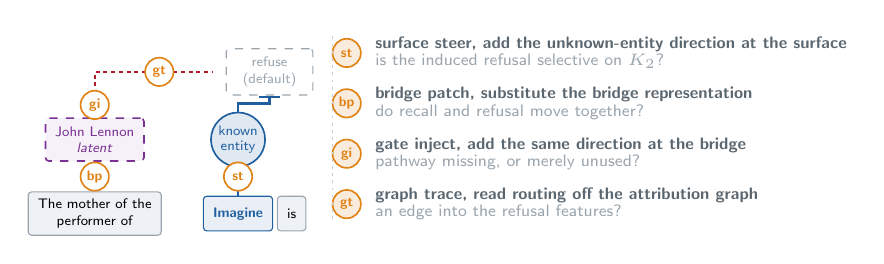
\begin{tikzpicture}
% ---------------- circuit skeleton ----------------
\node[tok, font=\sffamily\fontsize{5.2}{6}\selectfont] (m1) at (0.80,0.12) {The mother of the\\performer of};
\node[entity, font=\sffamily\bfseries\fontsize{5.2}{6}\selectfont] (m2) at (2.62,0.12) {Imagine};
\node[tok, font=\sffamily\fontsize{5.2}{6}\selectfont] (m3) at (3.30,0.12) {is};
\node[latentbox, font=\sffamily\fontsize{5.2}{6}\selectfont] (ml) at (0.80,1.06) {John Lennon\\\emph{latent}};
\node[gate, minimum size=6.0mm, font=\sffamily\fontsize{5}{5.5}\selectfont] (mg) at (2.62,1.06) {known\\entity};
\node[brakeoff, minimum width=1.1cm, font=\sffamily\fontsize{5.2}{6}\selectfont] (mb) at (3.02,1.92) {refuse\\(default)};
\draw[flow] (m2) -- (mg);
\draw[flowlat] (m1) -- (ml);
\draw[inhibit] (mg.north) -- (2.62,1.52) -- (3.02,1.52) -- (mb.south);
\draw[missing] (ml.north) -- (0.80,1.92) -- (2.30,1.92);
% each badge sits on the edge it targets, masking the line rather than a node
\node[badge, minimum size=3.6mm, fill=white] at (2.62,0.59) {\textit{st}};
\node[badge, minimum size=3.6mm, fill=white] at (0.80,0.59) {\textit{bp}};
\node[badge, minimum size=3.6mm, fill=white] at (0.80,1.50) {\textit{gi}};
\node[badge, minimum size=3.6mm, fill=white] at (1.62,1.92) {\textit{gt}};

% ---------------- interventions, two columns ----------------
\begin{scope}[xshift=4.00cm]
\foreach \y/\c/\a/\b in {
  2.16/{\textit{st}}/{surface steer, add the unknown-entity direction at the surface}/{is the induced refusal selective on $K_2$?},
  1.52/{\textit{bp}}/{bridge patch, substitute the bridge representation}/{do recall and refusal move together?},
  0.88/{\textit{gi}}/{gate inject, add the same direction at the bridge}/{pathway missing, or merely unused?},
  0.24/{\textit{gt}}/{graph trace, read routing off the attribution graph}/{an edge into the refusal features?}}
{
  \node[badge, minimum size=3.6mm] at (0,\y) {\c};
  \node[skctiny, text=skcSlate, anchor=west, font=\sffamily\bfseries\fontsize{5.6}{6.6}\selectfont] at (0.24,\y+0.11) {\a};
  \node[skctiny, text=skcMute, anchor=west, font=\sffamily\fontsize{5.6}{6.6}\selectfont] at (0.24,\y-0.11) {\b};
}
\end{scope}
\draw[draw=skcMute!55, line width=0.4pt, dash pattern=on 1pt off 1.6pt] (3.82,0.05) -- (3.82,2.40);
\end{tikzpicture}}
\vspace{-0.3em}
\caption{\textbf{The causal design.} All four interventions act on the same circuit, shown once at
left with each marked at the position it targets. Surface steer and gate inject add the
unknown-entity direction at the surface and bridge positions, bridge patch substitutes the bridge
representation from a matched query with an unknown bridge, and graph trace reads routing off the
computational graph \citep{ameisen2025circuittracing,hanna2025circuittracer}, validated by
intervention \citep{lindsey2025biology}. Bridge patch was designed to be decisive, since a change in recall without a matching change in
refusal is a double dissociation. \textbf{On the models tested the refusal arm is inert at baseline,
so the design did not deliver} (Section~\ref{sec:res-causal}). Protocol in
Appendix~\ref{app:controls}.}
\label{fig:causal}
\end{figure}


Four interventions separate the competing explanations, specified in full in
Table~\ref{tab:causal}, Appendix~\ref{app:controls}. Surface steer steers the unknown-entity direction at the
surface position and asks whether the induced refusal is selective on $K_2$. Bridge patch is the decisive
behavioral test. It patches the bridge representation from a matched query with an unknown bridge, and
measures the change in recall and in refusal on the same queries. A change in recall with no
matching change in refusal is a double dissociation. Gate inject injects the unknown-entity direction at the
\emph{bridge} position, distinguishing a missing routing pathway from an unused one, which decides
whether a repair must add routing or only supply a signal. Graph trace makes ``not routed'' a directly
measured property of the computational graph rather than an inference from behavior, using
attribution graphs over transcoders \citep{ameisen2025circuittracing,hanna2025circuittracer}.
Following \citet{lindsey2025biology}, every graph-derived claim is validated by intervention in the
underlying model, because the graph describes a replacement model.
% =====================================================================

Controls, protocol and status. (a) Named-bridge control, where the gap must close. \textbf{Run}, the
gap closes and reverses direction on both models tested, Gemma 2 2B (AUROC$(\gate\!\to\!K_2)=0.777$
composed vs.\ $0.895$ named-bridge, gap $+0.118$) and Llama 3.1 70B (gap $+0.155$, composed $0.637$
vs.\ named-bridge $0.793$, larger than Gemma 2 2B's). (b) Popularity-matched subsets by
pageview decile. \textbf{Run}, as bridge patch's own donor-matching methodology (192 pairs across 10 deciles on
the test split), not as a separate ablation with its own metric. (c) Length-matched distractor
control, substituting an unrelated real city for the true bridge in the named-bridge template,
length-matched toward the true prompt, and checking whether AUROC$(\gate\!\to\!K_2)$ collapses toward
chance. \textbf{Run}, distractor AUROC$=0.531$ (chance), versus control (a)'s real named-bridge
AUROC$=0.895$, so the gate reads the true bridge's own properties, not merely that some city is
named at that position. (d) Agreement across all three gate estimators. \textbf{Run}, and extended to a full 26-layer refit
sweep on Gemma 2 2B, refitting fresh diffmeans/probe/SAE gates independently at every layer with the
same protocol as layer 8, zero of 26 layers clear the full stop-gate. Difference-of-means and the
probe are both consistently strong (AUROC $0.75$--$0.89$ and $0.71$--$0.90$) and agree with each other
($\ge0.50$ Spearman) at $9$ of the $26$ layers, but the SAE estimator is weaker throughout
($0.44$--$0.85$ AUROC) and sets the minimum pairwise agreement at $23$ of the $26$ layers, with a
negative diffmeans--SAE correlation at 8 layers and a negative probe--SAE correlation at 2 more, so no
layer has all three agreeing simultaneously. This is a property of the SAE estimator on this model,
not a layer-choice problem, since switching layers changes which pair disagrees least, not whether a
layer exists where all three agree. (e)
Attention control, verifying the bridge position receives substantial attention, so a
failure to gate is not explained by the position being ignored. \textbf{Run}, mean attention from the
final prompt token to the bridge position is $0.112$, $1.82\times$ the $0.062$ a position would
receive under a uniform (ignored-position) null, so the position is attended, licensing the
``present but unread'' reading over ``simply ignored.'' (f) Random-direction negative
control, where a direction of matched norm drawn at random must produce no effect in surface steer, bridge
patch, or gate inject. \textbf{Run} on both Gemma 2 2B and Llama 3.1 70B, both the real and random
directions produce a refusal rate of exactly $0.000$ on both models, so this control is uninformative
on this model/template rather than passing or failing, since neither model exhibits refusal-lexicon
behavior on this template at all. Surface steer's own refusal rate was $0.000$ at every coefficient in
the validation sweep $\{-4,-2,-1,1,2,4,8\}$, split by $M$ or not, and gate inject and bridge patch's
baseline and patched generations show the same pattern. Sampled generations confirm this is not a
refusal-lexicon detection gap, since Gemma 2 2B at layer 8 states a confident answer and continues
with unrelated filler even when the answer is wrong (e.g.\ substituting a confabulated surname with
identical confidence to the correct one), rather than hedging (Section~\ref{sec:res-causal}).
(g) Counterfactual chains, so memorized composites cannot drive the result, substituting a false
premise for the true bridge fact and checking whether the model tracks the stated premise
(``composed'') or falls back to the real, memorized fact (``memorized''). \textbf{Run},
$p_{\mathrm{composed}}=0.732$ versus $p_{\mathrm{memorized}}=0.021$ ($n=239$, $p_{\mathrm{composed}}$
roughly $35\times$ $p_{\mathrm{memorized}}$), strong evidence against memorized composites driving
the paper's two-hop result. (h) Label validation against an {LLM} judge (Gemma 2 9B
instruction-tuned, $n=100$), reporting agreement. \textbf{Run}, agreement $=0.81$ on Gemma 2 2B and
$0.65$ on Llama 3.1 70B, with the same one-sided asymmetry on both (exact match scores items correct
that the judge scores wrong, $19$ on Gemma 2 2B, $35$ on Llama 3.1 70B, never the reverse). Exact
match is systematically more lenient than the judge, and more so on the larger model, plausibly
tracking its more varied phrasing rather than a labeling artifact specific to either model. (i)
Template and paraphrase robustness, following the
formatting sensitivity reported by \citet{tamoyan2025factual}, measures AUROC$(\gate\!\to\!K_2)$
stability across the original template and two genuine paraphrases (same entity-late, fixed-ending
clause structure). \textbf{Run}, $0.607$ (original), $0.618$ and $0.620$ (paraphrases), spread across
all three $=0.013$, essentially stable, not an artifact of one specific phrasing. (j) Cross-type
generalization, fitting the
gate on one entity type and the bridge readout on one relation type, then testing on held-out types.
\textbf{Partially run}, the entity-type half is done, leave-one-entity-type-out across all four
types (player, movie, city, song), comparing against an in-distribution reference fit on the same
population. Difference-of-means generalizes well (within $0.06$--$0.08$ AUROC of the in-distribution
reference for every type, and slightly exceeding it for player, $0.815$ vs.\ $0.799$), while the probe
generalizes far more unevenly (city drops to $0.559$ vs.\ a $0.846$ reference, near chance). The
relation-type half remains a genuine, disclosed data gap, since the two-hop dataset has exactly one
relation pair (place-of-birth$\to$country) across all $3503$ items, so there is nothing to hold out on
that side with the currently released data.
(k) Instruction-tuned versus base, and reasoning-tuned models, where
\citet{kirichenko2025abstentionbench} report that reasoning fine-tuning \emph{degrades} abstention, a
prediction that competes with ours in Section~\ref{sec:res-cot}. Instruction-tuned Gemma 2 9B is
already used for the chain-of-thought experiment above, so that half of (k) has a real result, while
the reasoning-tuned comparison does not. (l) Scale, a probe-based analysis on 32B (Qwen3-32B) and 70B (Llama 3.1 70B), both run, with
Qwen3-32B's own disclosed positive-control-disagreement caveat throughout (Table~\ref{tab:gap}, Section~\ref{sec:results}).
(m) Faithfulness, the fraction of graph-derived claims in graph trace that survive intervention
in the underlying model. Forty raw attribution graphs (20 queries, composed and named-bridge each)
have been built with circuit-tracer, but no refusal feature has been identified to score
edge weight into, since circuit-tracer's own released dictionaries carry no pre-labeled refusal feature,
identifying one is separate interpretability research the library does not provide, and this model
shows exactly $0.000$ refusal rate on this template at every coefficient tried (Section~\ref{sec:results}), leaving no
observed refusal behavior to correlate candidate features against in the first place. (m) remains
open pending that unresolved step, not pending a re-run. (n) Artifact probe, a
text-similarity-only detector that never sees model internals, after the TXTEMB baseline of
\citet{hussain2026parallax}, must sit at chance on our data. \textbf{Run}, and it does not pass. Text similarity alone predicts $Y$ at AUROC$=0.159$, which is
$0.341$ away from chance. Detection is sign-symmetric, so a detector that anti-predicts at $0.159$ is
a detector that predicts at $0.841$ once its sign is fixed, higher than every internal-state selector
in Table~\ref{tab:bgr-full} including ours. The mitigating detail is real but partial: $88\%$ of items
($211/239$) have zero prompt-target overlap and the signal comes from the remaining $28$, all
incorrect, so it is a narrow lexical correlation rather than an answer embedded in the prompt in the
sense \citet{hussain2026parallax} document. It is still the case that a model-free feature ranks these
items better than the internal states do, and a reviewer is entitled to ask what the internal-state
numbers add over it. \rf{re-run every selector in Table~\ref{tab:bgr-full} on the $211$-item
zero-overlap subset, and report whether BGR's margin over the surface gate survives there. Until that
exists, control (n) is a failed artifact check, and we label it so.}

\begin{center}
\small
\captionof{table}{\textbf{Does the written-position score see downstream hops?}
$n$ is held-out composed queries after the $K_1{=}1$ filter. Rows are ordered by parameter count so the
scale claim can be checked by eye. $D$ and $d$ (Kolmogorov--Smirnov, Cohen's $d$, negative meaning
composed queries score lower) compare the composed-query score distribution against the
single-hop-correct one; large values mean the distributions are far apart, so the pre-registered
overlap check \textbf{fails} on every model and the defensible claim is the weaker one in the AUROC
columns (Section~\ref{sec:res-blindspot}). The lower block misses on two counts: AUROC$(\gate\!\to\!M)$ departs from $\approx0.50$ on three models, and
$\widehat{\Delta}_{\mathrm{blind}}$ is exactly zero on two. No column carries a direction marker,
because lower slack and larger $\widehat{\Delta}_{\mathrm{blind}}$ favour this paper's reading rather
than being better in any external sense. \rf{bootstrap intervals on all nine columns. Every value here
is a point estimate from a single run, so no between-model comparison in this table is resolvable
(Appendix~\ref{app:power}).}}
\label{tab:gap}
\vspace{1pt}
\resizebox{\columnwidth}{!}{%
\begin{tabular}{@{}l r S[table-format=1.3] S[table-format=1.3] S[table-format=1.3] S[table-format=1.3] S[table-format=1.3] S[table-format=1.3] S[table-format=-1.3]@{}}
\toprule
& & \multicolumn{2}{c}{\textbf{AUROC}} & \multicolumn{2}{c}{\textbf{Slack}}
& \textbf{Blind} & \multicolumn{2}{c}{\textbf{Distribution shift}}\\
\cmidrule(lr){3-4}\cmidrule(lr){5-6}\cmidrule(lr){7-7}\cmidrule(l){8-9}
\textbf{Model} & {$n$} & {$\gate\!\to\!K_1$} & {$\gate\!\to\!M$} & {$\hat\delta$} &
{$\hat v$} & {$\widehat{\Delta}_{\mathrm{blind}}$} & {$D$} & {$d$}\\
\midrule
Gemma 2 2B                & 239 & 0.808 & 0.616 & 0.179 & 0.400 & 0.142 & 0.637 & -1.415\\
Llama 3.1 8B              & 350 & 0.711 & 0.320 & 0.160 & 0.328 & 0.000 & 0.905 & -3.030\\
Gemma 2 9B                & 346 & 0.828 & 0.375 & 0.170 & 0.063 & 0.191 & 0.792 & -2.178\\
Qwen3-32B$^{\dagger\S}$   &  97 & 0.831 & 0.580 & 0.069 & 0.119 & 0.000 & 0.823 & -1.892\\
Llama 3.1 70B$^{\dagger}$ & 494 & 0.775 & 0.561 & 0.102 & 0.275 & 0.049 & 0.738 & -2.150\\
\midrule
\multicolumn{9}{@{}l}{\emph{Predicted before measurement, if the written positions carry\ldots}}\\
\quad \ldots nothing about downstream hops & {--} & {high} & {$\approx0.50$} & {$\approx0$} & {$\approx0$} & {large} & {small} & {small}\\
\quad \ldots what the composed query needs  & {--} & {high} & {high} & {large} & {n/a} & {$\approx0$} & {--} & {--}\\
\bottomrule
\end{tabular}}

\vspace{2pt}
{\footnotesize $^{\dagger}$Difference-of-means and probe estimators only, since no public sparse
autoencoder exists for this model. The bridge-resolution filter is disabled throughout, for every
model (Section~\ref{sec:results}).
$^{\S}$Qwen3-32B is at layer 24, carrying its own positive-control stop-gate failure
(Table~\ref{tab:e0-allmodels}), reported anyway rather than dropped.}
\vspace{-0.7em}
\end{center}

\begin{center}
\small
\captionof{table}{\textbf{Positive control across models.} Diffmeans/probe AUROC on held-out
single-hop prompts, their cross-estimator agreement, and whether the stop-gate opens ($\ge0.65$ AUROC
each, $\ge0.50$ agreement). \textbf{No model clears the pre-registered three-estimator criterion};
every reported agreement is diffmeans--probe, with the sparse-autoencoder estimator excluded where one
exists (Gemma 2 2B/9B, Llama 3.1 8B) or unavailable ($^\dagger$, no public dictionary).
$^\S$Qwen3-32B is at its best layer (24), after a retry from layer 8 left agreement essentially
unchanged ($0.297\to0.296$), and clears neither criterion. \rv{this is a protocol asymmetry: four
models are read at a layer chosen once and never re-tuned, and one is read at its searched best layer.
Either sweep all five or report Qwen3-32B at layer 8 like the rest.}}
\label{tab:e0-allmodels}
\vspace{1pt}
\begin{tabular}{@{}l c S[table-format=1.3] S[table-format=1.3] S[table-format=1.3] c@{}}
\toprule
& & \multicolumn{2}{c}{\textbf{AUROC}} & &\\
\cmidrule(lr){3-4}
\textbf{Model} & \textbf{Layer} & {\textbf{Diffmeans}} & {\textbf{Probe}} &
{\textbf{Agreement}} & \textbf{Clears}\\
\midrule
Gemma 2 2B                & 8  & 0.886 & 0.887 & 0.547 & yes\\
Llama 3.1 8B              & 8  & 0.853 & 0.827 & 0.613 & yes\\
Gemma 2 9B                & 8  & 0.861 & 0.824 & 0.534 & yes\\
Qwen3-32B$^\S$            & 24 & 0.907 & 0.882 & 0.296 & \textbf{no}\\
Llama 3.1 70B$^\dagger$   & 8  & 0.771 & 0.752 & 0.514 & yes\\
\bottomrule
\end{tabular}
\end{center}

\begin{figure}[tb]
\centering
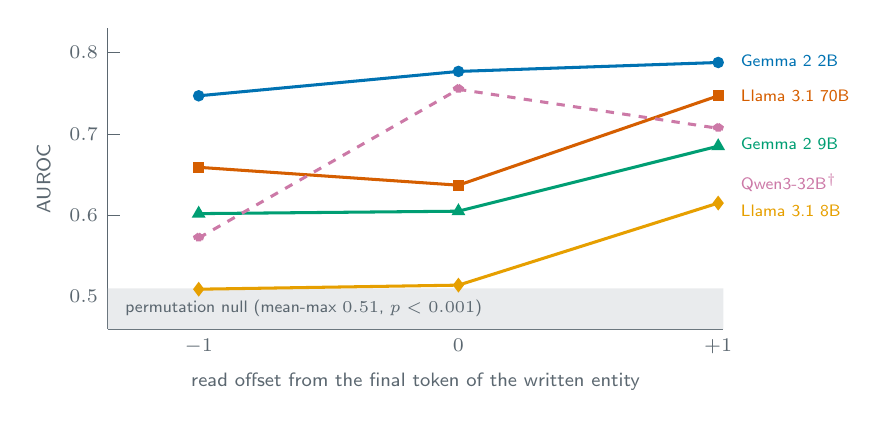
\begin{tikzpicture}
\definecolor{wBlue}{HTML}{0072B2}\definecolor{wVerm}{HTML}{D55E00}
\definecolor{wGrn}{HTML}{009E73}\definecolor{wOrg}{HTML}{E69F00}
\definecolor{wPur}{HTML}{CC79A7}
\begin{axis}[
  width=9.4cm, height=5.4cm,
  xlabel={read offset from the final token of the written entity},
  ylabel={AUROC},
  xmin=-1.35, xmax=1.02, ymin=0.46, ymax=0.83,
  xtick={-1,0,1}, xticklabels={$-1$,$0$,$+1$},
  ytick={0.5,0.6,0.7,0.8},
  axis line style={draw=skcSlate, line width=0.5pt},
  tick style={draw=skcSlate},
  tick label style={font=\sffamily\scriptsize, text=skcSlate},
  label style={font=\sffamily\scriptsize, text=skcSlate},
  axis x line*=bottom, axis y line*=left,
  clip=false, enlarge x limits=false,
]
% permutation null: mean-max over shuffles, the same reference for every series
\addplot[draw=none, fill=skcMute!22, forget plot]
  coordinates {(-1.35,0.46) (1.02,0.46) (1.02,0.51) (-1.35,0.51)} \closedcycle;
\node[skctiny, text=skcSlate, anchor=west] at (axis cs:-1.32,0.485) {permutation null (mean-max $0.51$, $p<0.001$)};

\addplot[wBlue, line width=1.1pt, mark=*,        mark size=1.5pt] coordinates {(-1,0.747)(0,0.777)(1,0.788)};
\addplot[wVerm, line width=1.1pt, mark=square*,  mark size=1.4pt] coordinates {(-1,0.659)(0,0.637)(1,0.747)};
\addplot[wGrn,  line width=1.1pt, mark=triangle*,mark size=1.8pt] coordinates {(-1,0.602)(0,0.605)(1,0.685)};
\addplot[wOrg,  line width=1.1pt, mark=diamond*, mark size=1.8pt] coordinates {(-1,0.509)(0,0.514)(1,0.615)};
\addplot[wPur,  line width=1.1pt, mark=pentagon*,mark size=1.5pt, dashed] coordinates {(-1,0.572)(0,0.755)(1,0.707)};

\node[skctiny, text=wBlue, anchor=west] at (axis cs:1.05,0.790) {Gemma 2 2B};
\node[skctiny, text=wVerm, anchor=west] at (axis cs:1.05,0.747) {Llama 3.1 70B};
\node[skctiny, text=wGrn,  anchor=west] at (axis cs:1.05,0.688) {Gemma 2 9B};
\node[skctiny, text=wPur,  anchor=west] at (axis cs:1.05,0.640) {Qwen3-32B$^{\dagger}$};
\node[skctiny, text=wOrg,  anchor=west] at (axis cs:1.05,0.606) {Llama 3.1 8B};
\end{axis}
\end{tikzpicture}
\vspace{-0.4em}
\caption{\textbf{The frozen direction is readable one token past the written entity.} AUROC for the
direction fit on one-hop data and never refit, read at three offsets around the bridge-resolution
position, at the layer where each model's own gate is trustworthy.
\rf{the target these AUROCs are computed against. The manuscript never states whether the sweep scores
$K_2$, $M$ or $Y$, and the figure cannot label its own axis until it does.} Every peak clears
the permutation null comfortably, and four of five models peak at offset $+1$, which is the position
BGR reads. Single runs with no seed variation and no confidence intervals
(Appendix~\ref{app:power}), so the ordering between models should not be read as resolved.
$^{\dagger}$Qwen3-32B is at layer 24 and carries the positive-control failure of
Table~\ref{tab:e0-allmodels}; it is the one model peaking at offset $0$.}
\label{fig:offsets}
\end{figure}


Protocol for the compounding experiment. Repeat the blind-spot analysis on family F2, comparing each
three-hop chain against \emph{its own} two-hop
prefix rather than a separate two-hop set, so $M_2$ and $M_3$ live on the same items and the
monotonicity clause applies. Estimate $\mathbb{P}(M_k=0)$, $\delta_k$, $v_k$ and the floor for
$k=2,3$, and report whether the floor rises and whether the slack terms rise faster. Gemma 2 2B's own
result is in Section~\ref{sec:results}, and Table~\ref{tab:compound-allmodels} gives the same check on
four more models.

\begin{center}
\small
\captionof{table}{\textbf{Leading term, floor and slack at $k{=}2$ against $k{=}3$.} $n$ is retained
three-hop chains after the $K_1{=}1$ filter; rows ordered by parameter count. Adjacent columns rather
than in-cell arrows, so the change can be read down as well as across. \textbf{A floor of $0.000$ is a
negative raw bound clipped at zero, a vacuous bound and not a bound of zero}; the raw $k{=}2$ values
are $-0.457$, $-0.270$, $-0.211$, $+0.009$ and $-0.008$ in row order, so only Qwen3-32B is even
nominally positive there. $^{\ast}$Gemma 2 2B is the model discussed in
Section~\ref{sec:results}, included so all five are comparable in one place. $^\dagger$Layer 24,
carrying the positive-control failure of Table~\ref{tab:e0-allmodels}.}
\label{tab:compound-allmodels}
\vspace{1pt}
\begin{tabular}{@{}l r S[table-format=1.3] S[table-format=1.3] S[table-format=1.3] S[table-format=1.3] S[table-format=1.3] S[table-format=1.3]@{}}
\toprule
& & \multicolumn{2}{c}{$\mathbb{P}(M{=}0)$} & \multicolumn{2}{c}{\textbf{Floor}}
& \multicolumn{2}{c}{$\delta_k+v_k$}\\
\cmidrule(lr){3-4}\cmidrule(lr){5-6}\cmidrule(l){7-8}
\textbf{Model} & {$n$} & {$k{=}2$} & {$k{=}3$} & {$k{=}2$} & {$k{=}3$} & {$k{=}2$} & {$k{=}3$}\\
\midrule
Gemma 2 2B$^{\ast}$ & 252 & 0.476 & 0.845 & 0.000 & 0.135 & 0.933 & 0.710\\
Llama 3.1 8B        & 405 & 0.178 & 0.560 & 0.000 & 0.013 & 0.448 & 0.548\\
Gemma 2 9B          & 452 & 0.400 & 0.476 & 0.000 & 0.325 & 0.611 & 0.151\\
Qwen3-32B$^\dagger$ &  87 & 0.207 & 0.471 & 0.009 & 0.067 & 0.198 & 0.404\\
Llama 3.1 70B       & 731 & 0.439 & 0.466 & 0.000 & 0.052 & 0.447 & 0.415\\
\bottomrule
\end{tabular}

\vspace{2pt}
{\footnotesize $^\dagger$Layer 24, carrying the standing positive-control caveat
(Section~\ref{sec:res-e0}). In every case the leading term and floor rise together with $k$, as the
theorem's own remark permits regardless of which way slack moves. Slack itself falls for Gemma 2
9B/Llama 3.1 70B and grows for Llama 3.1 8B/Qwen3-32B, so growing slack is not unique to the one
model carrying the standing positive-control caveat.}
\end{center}

Protocol for the chain-of-thought experiment. On family F3, prompt with chain of thought so the model
writes the bridge itself, read the
gate at the self-written mention, and compare against the same items answered directly. Report AUROC
against $K_2$ and abstention quality, split by whether the written bridge is correct. Results for
Gemma 2 9B instruction-tuned and Llama 3.1 8B Instruct are in Section~\ref{sec:res-cot}. The full split, with the
direct-answer references of $0.369$ and $0.516$, is in Section~\ref{sec:res-cot}.
\rf{a paired test on the correct-versus-wrong contrast with bootstrap intervals on each arm. Until it
exists this reports a direction, not a result, and cannot be cited against
\citet{cheng2025cotobscures}.} Both models
tested are instruction-tuned; Gemma 2 2B did not clear the positive control's agreement bar at any of
three attempted layer and sample-size combinations. The heavy arm imbalance ($44$ against $889$, $46$
against $3075$) reflects how rarely chain of thought both names a bridge and gets it right on family
F1. Abstention quality under this split is a selective-risk/AURC-style curve that the released harness
does not yet compute, and it is not yet run.

Three of the controls above are load-bearing. Counterfactual chains, without which memorized
composites can produce the effect, are run ($p_{\mathrm{composed}}=0.732$ vs.\ $p_{\mathrm{memorized}}=0.021$,
see above). The
random-direction negative control, without which any intervention result is uninterpretable, is run
and is uninformative on this model/template rather than passing, since neither arm produces any
refusal at all (see above). Cross-type generalization, without which the readout may be
relation-specific, is partially run, with the entity-type half done and the relation-type half a
disclosed data gap (see above). Two of the three are therefore not in the state the design required,
and the causal claims that depend on them are withdrawn in Section~\ref{sec:res-causal} rather than
carried.

Controls (f), (g), and (j) are the ones whose omission would leave a reviewer unable to distinguish
our claim from a frequency effect, an intervention artifact, or a relation-specific fit. Control (m)
follows \citet{lindsey2025biology}. An attribution graph describes a replacement model, so a
graph-derived claim is not evidence until it survives intervention in the underlying model, and we
report the survival rate rather than only the claims that survived.

\section{Estimating the slack terms}
\label{app:estimation}
% =====================================================================

Two estimation points, both found by running the released smoke test on synthetic data with known
ground truth.

First, the non-negativity of $\Delta_{\mathrm{blind}}$ and $\Delta_{\mathrm{subopt}}$ is a statement
about population quantities. Both are estimated with cross-fitted plug-ins for $R^\ast$, so fold-wise
calibration differences can drive an estimated term slightly negative even where the identity holds;
on synthetic data the violations sit near a tenth of a binomial standard error. The released code
tolerates violations inside sampling noise, reports them, and raises on anything larger, because a
large negative term signals an estimation fault rather than a finding.

Second, one natural estimation choice is wrong rather than conservative. Substituting the
\emph{marginal} rate $\mathbb{P}(Y=1,K_2=0)$ for $v$ under-estimates the essential supremum whenever
the gate carries information about $K_1$, because shortcut answers concentrate where the gate fires.
That raises the computed floor above its true value and can manufacture an apparent violation of
Theorem~\ref{thm:floor} on data where it holds: on the same synthetic data the marginal estimator
reported a violation and the conditional estimator did not. The code refuses the marginal estimator by
default and a regression test pins the behavior. The same applies to $\delta$, $\delta_k$ and $v_k$.
Relatedly, comparing the floor against the minimum of the empirical risk-coverage curve false-alarms,
because the minimum over many correlated thresholds is biased downward, so we flag a violation only
when the one-sided upper confidence limit of the empirical risk lies strictly below the floor.

% =====================================================================
\section{What this sample size can resolve}
\label{app:power}
% =====================================================================

Every comparison in the paper runs on $n{=}239$ held-out composed items (Llama 3.1 70B, $n{=}494$).
Hanley--McNeil standard errors on that design, using the class balance implied by
$\mathbb{P}(M{=}0)=0.439$ for $K_2$ labels and by control~(n) for $Y$ labels, give the resolution
in Table~\ref{tab:power}. This appendix exists because several comparisons in earlier drafts were
smaller than the noise and were stated as findings anyway.

\begin{center}
\small
\captionof{table}{\textbf{Resolvable and unresolvable comparisons at $n{=}239$.} Paired intervals
assume a between-condition rank correlation of $0.5$; the true correlation is not reported, which is
itself a gap.}
\label{tab:power}
\vspace{1pt}
\begin{tabular}{@{}lccl@{}}
\toprule
\textbf{Comparison} & \textbf{Effect} & \textbf{95\% CI} & \textbf{Verdict}\\
\midrule
BGR-min vs surface gate ($Y$) & $+0.204$ & $\pm0.084$ & resolvable, and unpaired too\\
Named vs composed, Gemma 2 2B ($K_2$) & $+0.118$ & $\pm0.051$ & resolvable\\
Gap on 70B vs gap on 2B & $+0.037$ & $\pm0.094$ & \textbf{not resolvable}\\
BGR gain on 70B & $+0.082$ & $\pm0.06$ & marginal\\
\midrule
\multicolumn{4}{@{}l}{\emph{Minimum detectable AUROC difference, $80\%$ power, $\alpha=0.05$}}\\
\quad unpaired & -- & $0.189$ & \\
\quad paired, $\rho=0.5$ & -- & $0.134$ & \\
\bottomrule
\end{tabular}
\end{center}

Two consequences. Any AUROC difference below roughly $0.13$ on this set is not something the
experiment can speak to, which rules out most cross-model and most baseline-versus-baseline
statements. And the two comparisons that do survive are the two the paper now leads with, which is the
right outcome but was not by design.
\rf{the actual paired rank correlation between conditions, so these intervals can be replaced by
measured ones rather than assumed ones, and a pre-registered minimum-detectable-effect calculation for
any comparison added in future work.}

% =====================================================================
\section{Claim-to-experiment map}
\label{app:map}
% =====================================================================

Table~\ref{tab:map} lists every claim the paper makes, the experiment that is supposed to support it,
and its status. Rows marked \emph{open} are experiments the paper needs and does not have; they are
design gaps, not merely unfilled numbers.

\begin{center}
\small
\captionof{table}{\textbf{Claim-to-experiment map.} $n$ is models the experiment was run on, of five.
CI means bootstrap intervals are reported for that experiment.}
\label{tab:map}
\vspace{1pt}
\resizebox{\columnwidth}{!}{%
\begin{tabular}{@{}p{5.1cm}p{4.3cm}ccp{3.1cm}@{}}
\toprule
\textbf{Claim} & \textbf{Experiment} & $n$ & \textbf{CI} & \textbf{Status}\\
\midrule
The gate is trustworthy where the entity is written & Positive control, held-out single-hop AUROC & 5 & yes & three-estimator bar not met by any model\\
\addlinespace[2pt]
The gate separates $K_1$ but not $Y$ & AUROC on $n{=}239$ composed & 5 & \textbf{no} & class balance unstated\\
\addlinespace[2pt]
Part of the shortfall is availability, not scoring & Named-bridge comparison & 2 & \textbf{no} & \emph{open} on three models\\
\addlinespace[2pt]
The gap is the referent, not the position & Length-matched distractor & 1 & \textbf{no} & \emph{open} on four models\\
\addlinespace[2pt]
Writing the referent changes ranking, not just level & Score-level shift, composed vs named & 0 & -- & \emph{open} \citep{lathkar2026anchored}\\
\addlinespace[2pt]
The latent state is linearly present & Offset sweep vs permutation null & 5 & no & split for peak selection unstated\\
\addlinespace[2pt]
Reading it recovers availability & BGR vs 13 baselines & 2 & partial & \emph{open} on three models; DRIFT not run\\
\addlinespace[2pt]
The gain comes from the conjunction & \textbf{Bridge-only, mean, max arms} & 0 & -- & \emph{open}, see below\\
\addlinespace[2pt]
The benchmark does not leak the answer & Text-only artifact probe & 1 & no & \textbf{failed}; zero-overlap re-run \emph{open}\\
\addlinespace[2pt]
Not driven by memorized composites & Counterfactual chains & 1 & no & passed\\
\addlinespace[2pt]
Not a phrasing artifact & Three paraphrases & 1 & no & passed\\
\addlinespace[2pt]
Not explained by an ignored position & Attention to bridge position & 1 & no & passed\\
\addlinespace[2pt]
Not relation-specific & Cross-type generalization & 1 & no & entity-type half only; \emph{open} on relations\\
\addlinespace[2pt]
The effect is not a small-model artifact & Five models, $35\times$ range & 5 & no & $\widehat{\Delta}_{\mathrm{blind}}{=}0$ on two\\
\addlinespace[2pt]
The bound becomes informative with depth & $k{=}2$ vs $k{=}3$ & 5 & no & vacuous at $k{=}2$ on four\\
\addlinespace[2pt]
The method is cheap & Forward-pass count only & 5 & -- & \emph{open}: no timing, no memory\\
\addlinespace[2pt]
Refusal is gated by the written entity & Four causal interventions & 2 & -- & \textbf{all degenerate}, claim withdrawn\\
\bottomrule
\end{tabular}}
\end{center}

\paragraph{The single most important open experiment.} \rf{a \textbf{bridge-only} arm: score with
$g_{\bridge}$ alone and report it next to BGR-min in Table~\ref{tab:bgr}. Every claim about the
\emph{conjunction} rests on it. If $g_{\bridge}$ alone reaches roughly BGR-min's $0.766$, the finding
is ``read at a different position,'' the minimum contributes nothing, and Section~\ref{sec:bgr}'s
motivation is wrong. If it lands well below and the minimum recovers the difference, the conjunction
is doing the work. This is one line of analysis code on data already collected, it is the cheapest
experiment in this table, and it can falsify the method's design rationale.}

\paragraph{Two more that are cheap on existing data.} \rf{a risk-coverage curve for the surface gate,
BGR-min, and the strongest baseline on the $n{=}239$ set. The paper's central object is selective risk
at a coverage and it currently reports only three points from that curve.} \rf{a failure analysis:
sample the composed items where BGR-min answers and is wrong, and where it abstains and would have
been right, and report what distinguishes them. There is no qualitative analysis in the paper at all.}

\paragraph{Generality is the schedule driver.} \rf{at least six composable relation pairs, screened
for bridge guessability with the procedure of \citet{yang2024shortcuts}. The released two-hop set uses
\emph{place of birth $\to$ country}, which is one of exactly two relations that paper filters out
because the bridge is inferable from the head entity's surface form. Every availability number in this
paper is currently a number about that one relation, and the $\hat v=0.400$ shortcut rate is what that
looks like from the inside.}

% =====================================================================
\section{Extended setup}
\label{app:setup}

\paragraph{Compute.} \rf{hardware, total GPU-hours, and quantization details for every run. Nothing
about compute appears in the paper, and ICLR reviewers ask.} \rf{the license of each released
artifact (the released query sets, the code) and the license terms of the Wikidata, MuSiQue and 2WikiMultiHopQA
sources it derives from.}

\paragraph{Power.} A pre-registered minimum-detectable-effect calculation for the primary comparison
and the headline repair comparison, computed before collection rather than from the count the data
happened to provide, is a design step for the human authors and is not reported here.
\rf{the class balance of the held-out composed set. Every AUROC against $Y$ in
Tables~\ref{tab:bgr} and \ref{tab:bgr-full} is computed on $n{=}239$ items whose positive/negative
split is never stated; the control (n) figures imply roughly 40 incorrect items, which would put wide
intervals on all thirteen baselines and on both BGR variants.} \rf{bootstrap confidence intervals on
every cell of Tables~\ref{tab:gap}, \ref{tab:bgr} and \ref{tab:bgr-full}. Only the positive control
currently carries intervals, so no comparison other than BGR-versus-surface-gate has an uncertainty
estimate.}
% =====================================================================

\begin{center}
\small
\captionof{table}{\textbf{The three query families.} F3 is the control that converts a latent referent into a written
one without changing the question. Counts are held-out items after the $K_1{=}1$ filter only; the
bridge-resolved filter is not applied anywhere in this paper (Section~\ref{sec:results}).}
\label{tab:bench}
\vspace{1pt}
\resizebox{\columnwidth}{!}{%
\begin{tabular}{@{}lllrl@{}}
\toprule
\textbf{Family} & \textbf{Latent entity is} & \textbf{Source} & \textbf{Items} & \textbf{Tests}\\
\midrule
F1 Bridge & the referent of a description & \citet{yang2024latent}, Wikidata & 239$^{\ddagger}$ & the base phenomenon\\
F2 Chain ($k{=}3$) & two intermediate referents & Wikidata compositions & 252$^{\ddagger}$ & compounding, Thm.~\ref{thm:floor}\\
F3 Self-written & written by the model in its own CoT & F1 with reasoning prompts & 933$^{\S}$ & whether writing restores gating\\
\bottomrule
\end{tabular}}
\vspace{1pt}
{\footnotesize $^{\ddagger}$Gemma 2 2B, layer 8, $K_1{=}1$ only (bridge-resolution filter disabled, no
independent Patchscopes confirmation, see Section~\ref{sec:results}).
$^{\S}$Gemma 2 9B instruction-tuned, $44$ with a correct self-written bridge, $889$ with an incorrect
one.}
\vspace{-1.15em}
\end{center}


\begin{center}
\small
\captionof{table}{\textbf{Causal design.} $\uparrow$ marks a predicted change, $\approx$ no change.
See Figure~\ref{fig:causal} for what each intervention does.}
\label{tab:causal}
\vspace{1pt}
\resizebox{\columnwidth}{!}{%
\begin{tabular}{@{}llccl@{}}
\toprule
& & \multicolumn{2}{c}{\textbf{Predicted}} &\\
\cmidrule(lr){3-4}
\textbf{Intervention} & \textbf{Read-out} & \textbf{Surface-only reading} & \textbf{Composed reading} & \textbf{What it settles}\\
\midrule
Surface steer    & refusal rate $\mid M{=}1$ & $\uparrow$   & $\approx$    & \multirow{2}{*}{is the induced refusal selective?}\\
                 & refusal rate $\mid M{=}0$ & $\uparrow$   & $\uparrow$   & \\
\addlinespace[3pt]
Bridge patch     & $\Delta$ recall           & $\downarrow$ & $\downarrow$ & \multirow{2}{*}{\textbf{decisive}, a double dissociation}\\
                 & $\Delta$ refusal rate     & $\approx$    & $\uparrow$   & \\
\addlinespace[3pt]
Gate inject      & refusal rate at bridge    & $\approx$    & $\uparrow$   & pathway absent, or present but unused\\
\addlinespace[3pt]
Graph trace      & edge weight to refusal    & $\approx 0$  & $\uparrow$   & routing as a graph property, not an inference\\
\bottomrule
\end{tabular}}
\vspace{1pt}
{\footnotesize Every read-out in the refusal column returned exactly $0.000$ at baseline and under
every intervention, so the predicted contrasts were not testable on these models
(Section~\ref{sec:res-causal}).}
\vspace{-1.15em}
\end{center}

\paragraph{Splits.} Entities are partitioned into fit and held-out sets by \emph{entity} rather than by
prompt, before anything is estimated. Gate directions are fit on single-hop prompts in the fit split
only; every number in Section~\ref{sec:results} comes from the held-out split.
\rv{whether the partition covers $b_1$ and $a$ or only $e_1$. This is the leakage vector that matters
here: if a test item's \emph{bridge} appeared as a written entity in a fit-split single-hop prompt,
the direction was fit on activations from that very referent and then read at its latent position, and
the transfer result is partly memorization. Confirm the partition is over the union
$\{e_1,b_1,a\}$, or re-split and re-report.}

\paragraph{Gate estimators.} (i) SAE latents are selected by the separation score of
\citet{ferrando2025entity}, taking the top latent per (layer, entity type) and then the latent
maximizing the minimum separation across types, which is the generalizing choice rather than the
best-fitting one. (ii) The difference-of-means direction is the normalized difference of mean
residual-stream activations between known and unknown entity groups at the same position.
(iii) The logistic probe is $\ell_2$-regularized, with the penalty chosen by five-fold
cross-validation \emph{within} the fit split. All three are read at the final token of the entity
mention, at layer 8 for every model except Qwen3-32B (layer 24). No public SAE dictionary exists for
Llama or Qwen3, so those models use difference-of-means and probe only.

\paragraph{Interventions.} Steering coefficients are selected on a validation split disjoint from
both fit and test, following \citet{ferrando2025entity}, and reported with the sweep rather than only
the chosen value. Patching replaces the residual stream at the bridge position across a contiguous
layer window. The window is selected by the frozen-direction sweep's own empirical peak (layer, position offset,
Section~\ref{sec:res-latent}) on the composed prompt and reported, not by the during-generation
Patchscopes site, since no composed-prompt position was found where Patchscopes decodes a clean
entity. \rv{whether that peak was selected on the validation split or on the held-out split. The
same ambiguity affects BGR's read position (Section~\ref{sec:bgr}) and is the single largest
reproducibility gap in the method.}
The coefficient sweep tried on Gemma 2 2B, layer 8, is $\{-4,-2,-1,1,2,4,8\}$, and the selected
coefficient is $-4$ (maximizing validation-split refusal rate, all of which were $0.000$, so no
non-degenerate selection criterion is possible here, since refusal never varies with coefficient on
this model/template combination). The layer window is $[7,10)$, centered on that sweep's peak layer.
The same sweep on Gemma 2 9B instruction-tuned, with the layer window centered on that model's own
peak (layer 8, the same window, $[7,10)$), gives a refusal rate that is again exactly $0.000$ at every
coefficient in $\{-4,-2,-1,1,2,4,8\}$, the same degenerate outcome as the base model, evidence the
null is about this refusal template rather than about instruction tuning specifically.

\paragraph{Refusal detection.} A response counts as a refusal if it matches a refusal lexicon
\emph{and} contains no candidate attribute string. Both conditions are required, because a response
can hedge and still commit to an answer. The lexicon is fixed in advance from the validation split
and released. A held-out manual audit against the automatic label, the one place the pipeline touches
human judgment, is a task for the human authors and its agreement rate is not reported here.
\rf{that agreement rate. It matters more than usual here, because the refusal rate is exactly $0.000$
everywhere and a detection gap in the lexicon is one of the two explanations for that null.}

\paragraph{Statistics.} \rf{seed variation. Every number in this paper comes from a single run.
Bootstrap over queries estimates sampling noise in the evaluation set; it says nothing about variance
from probe initialization, the cross-validation folds that pick the probe penalty, the cross-fitting
folds in BGR-lr, or sparse-autoencoder latent selection. Re-run the full pipeline under at least five
seeds and report seed standard deviation separately from the bootstrap interval. A paired-bootstrap
$p<0.001$ from one run does not establish that the comparison is stable across seeds.}
All intervals are percentile bootstrap over queries with 2{,}000 resamples,
resampling queries, not prompts, so the composed item and its decompositions move together. AUC comparisons use both a paired bootstrap and DeLong \citep{delong1988comparing}, and we
report both, since agreement between them is evidence that neither is being driven by an artifact of
its own assumptions. Multiplicity across relation types is controlled at the 5\% level by
Benjamini-Hochberg \citep{benjamini1995controlling}. Every $\kappa$ estimate is reported at
$\alpha\in\{0.01,0.05,0.10\}$.

\paragraph{Data provenance.} Wikidata has no versioned snapshot identifier for live SPARQL queries
against \lit{query.wikidata.org}, so we instead record the query date, which is what reproducing
the same pull requires. The two-hop query set (\lit{data/twohop\_queries.json}) was pulled
2026-08-11, the three-hop query set (\lit{data/threehop\_queries.json}, $n=3961$ chains) was
pulled 2026-08-26, and Wikipedia pageview counts (\lit{data/pageviews\_twohop.json}, monthly views
summed over 2024, all 847 bridge entities from the two-hop set resolved to a real article) were
pulled 2026-08-27 from the public Wikimedia Pageviews REST API. No additional model-specific query set
was pulled beyond these three, and all reported models score against this same fixed set.

% =====================================================================

\begin{center}
\small
\captionof{table}{\textbf{All thirteen baselines plus every BGR variant, both in-scope models.}
Gemma 2 9B (layer 8, $n{=}346$) and Llama 3.1 70B (layer 25, $n{=}494$), each the model's own
confirmed-stable positive-control layer. Every row is 5 seeds EXCEPT bridge-only/BGR-min/BGR-mean,
which are one seed (Section~\ref{sec:bgr}: their own $g_{\bridge}$ capture was corrected this pass and
has not yet been re-run across seeds). \emph{Audit} is the verdict of the controlled
re-run by \citet{hussain2026parallax}, where \checkmark{} exceeded chance once benchmark artifacts were
removed, $\times$ did not, and -- was not covered. Best per column within a tier and model is bolded.
\rv{only the SAPLMA \checkmark{} has been confirmed against the primary source, which names SAPLMA and
DRIFT as its two consistent exceptions. Confirm the \citet{kossen2024semantic} and
\citet{du2024haloscope} $\times$ verdicts against that paper's own method table before submission, or
mark them as not covered.}}
\label{tab:bgr-full}
\vspace{1pt}
\resizebox{\columnwidth}{!}{%
\begin{tabular}{@{}llc S[table-format=1.3] S[table-format=1.3] S[table-format=1.3] S[table-format=1.3] S[table-format=1.3] S[table-format=1.3]@{}}
\toprule
& & & \multicolumn{3}{c}{\textbf{Gemma 2 9B}} & \multicolumn{3}{c}{\textbf{Llama 3.1 70B}}\\
\cmidrule(l){4-6}\cmidrule(l){7-9}
\textbf{Selector} & \textbf{Cost} & \textbf{Audit} & {\textbf{AUROC}$\uparrow$} & {\textbf{AURC}$\downarrow$} & {\textbf{R@50\%}$\downarrow$} &
{\textbf{AUROC}$\uparrow$} & {\textbf{AURC}$\downarrow$} & {\textbf{R@50\%}$\downarrow$}\\
\midrule
\multicolumn{9}{@{}l}{\emph{One forward pass}}\\
\quad Surface gate \citep{ferrando2025entity}            & $1\times$ & -- & 0.352 & 0.512 & 0.601 & 0.484 & 0.552 & 0.543\\
\quad Semantic entropy probe \citep{kossen2024semantic}  & $1\times$ & $\times$ & 0.203 & 0.710 & 0.671 & 0.502 & 0.554 & 0.534\\
\addlinespace[3pt]
\multicolumn{9}{@{}l}{\emph{Extra passes or sampling}}\\
\quad $P(\text{True})$ \citep{kadavath2022know}          & $2\times$ & -- & 0.481 & 0.457 & 0.468 & 0.568 & 0.497 & 0.510\\
\quad SAPLMA \citep{azaria2023internal}                  & $2\times$ & \checkmark & 0.316 & 0.582 & 0.624 & 0.580 & 0.505 & 0.474\\
\quad Entity-level token probes \citep{obeso2025realtime}& $2\times$ & -- & 0.413 & 0.454 & 0.520 & 0.532 & 0.515 & 0.530\\
\quad Lookback Lens \citep{chuang2024lookback}           & $2\times$ & -- & 0.466 & 0.451 & 0.480 & \bfseries 0.670 & \bfseries 0.421 & \bfseries 0.417\\
\quad HaloScope \citep{du2024haloscope}                  & $2\times$ & $\times$ & 0.455 & 0.555 & \bfseries 0.399 & 0.458 & 0.574 & 0.587\\
\quad ICR probe \citep{zhang2025icrprobe}                & $2\times$ & -- & 0.266 & 0.619 & 0.618 & 0.633 & 0.463 & 0.441\\
\quad SelfCheckGPT \citep{manakul2023selfcheckgpt}       & $k{=}10$  & -- & 0.156 & 0.744 & 0.728 & 0.608 & 0.436 & 0.526\\
\quad Semantic entropy \citep{farquhar2024semantic}      & $k{=}10$  & -- & 0.442 & 0.518 & 0.497 & 0.541 & 0.504 & 0.547\\
\quad INSIDE \citep{chen2024inside}                      & $k{=}10$  & -- & \bfseries 0.538 & \bfseries 0.412 & 0.422 & 0.477 & 0.575 & 0.555\\
\addlinespace[3pt]
\multicolumn{9}{@{}l}{\emph{Multi-call decomposition}}\\
\quad Self-ask abstention \citep{press2023compositionality} & multi-call & -- & 0.500 & 0.480 & 0.491 & 0.500 & 0.541 & 0.547\\
\quad Operadic consistency \citep{bottman2026operadic}      & multi-call & -- & 0.500 & 0.480 & 0.491 & 0.500 & 0.541 & 0.547\\
\midrule
\multicolumn{9}{@{}l}{\emph{Ours, one forward pass}}\\
\quad \textbf{Bridge-only} (no aggregation rule)         & $1\times$ & -- & \bfseries 0.686 & \bfseries 0.324 & \bfseries 0.306 & \bfseries 0.606 & \bfseries 0.439 & \bfseries 0.413\\
\quad BGR-min (parameter-free conjunction)               & $1\times$ & -- & 0.415 & 0.467 & 0.543 & 0.506 & 0.502 & 0.502\\
\quad BGR-mean (parameter-free compensation)             & $1\times$ & -- & 0.490 & 0.416 & 0.462 & 0.548 & 0.492 & 0.457\\
\midrule
\multicolumn{9}{@{}l}{\emph{Ours, two features, cross-fitted}}\\
\quad \textbf{BGR-lr}                                    & $1\times$ & -- & \bfseries 0.827 & \bfseries 0.263 & \bfseries 0.179 & \bfseries 0.669 & \bfseries 0.414 & \bfseries 0.437\\
\midrule
\multicolumn{9}{@{}l}{\emph{Ceiling}}\\
\quad Oracle observing $M$ (reference)                   & --        & -- & 0.788 & 0.303 & 0.272 & 0.681 & 0.385 & 0.433\\
\bottomrule
\end{tabular}}

\vspace{1pt}
{\footnotesize All rows are from real runs on both models with a confirmed, five-seed-stable positive
control ($K_1{=}1$ only; Patchscopes does not independently confirm bridge resolution at either
model's own layer, disclosed and unchanged from Section~\ref{sec:results}).
\rf{this table on the three models WITHOUT a confirmed positive control (Gemma 2 2B, Llama 3.1 8B,
Qwen3 32B) -- not because the suite was never run on them, but because an exhaustive per-layer,
five-seed search found no layer at which any of the three clears the pre-registered agreement bar
(Section~\ref{sec:res-e0}). Reporting BGR/bridge-only numbers for those models would be reporting a
selector against an instrument known not to work.}
\rf{a multiplicity correction across the thirteen baselines. ``Best in tier'' and ``beats all but
one'' are selections over many comparisons and no correction is applied anywhere; the one specified in
the setup was across relation types, of which there is one.} Self-ask and Operadic consistency report
identical numbers at both models because both reduce to a constant score. \rv{\citet{bottman2026operadic}
evaluate operadic consistency over sampled decompositions and compare it against sample-based
self-consistency at matched call budget, whereas our run compares a single greedy direct answer against
a single greedy decomposed answer, which cannot vary. Re-run it with the sampling protocol of the
original paper or state in the table that the baseline is run outside its intended regime.} Both models
show exactly $0.000$ refusal rate at every coefficient tried (Section~\ref{sec:results}), so self-ask
never abstains, and Operadic consistency's direct-vs-decomposed answers never disagree under greedy
decoding on either non-hedging model, a real, shared consequence of that null, not a computation error
(confirmed against two independent runs and an analytic check that only a fully constant score
reproduces AUROC$=0.500$ to this precision).}
\vspace{-1.9em}
\end{center}

\section{Prompt templates}
\label{app:prompts}
% =====================================================================

Table~\ref{tab:templates} lists the templates. They place the entity late and end on a fixed token, following \citet{tamoyan2025factual}, whose
ablation found that this form avoids the spurious correlations that arise when the prompt ends on
variable tokens. Angle brackets mark slots.

\begin{center}
\small
\captionof{table}{\textbf{Prompt templates.} Matching and the distractor control are specified in
Section~\ref{sec:instrument}. Angle brackets mark slots; $b$ is the gold bridge $b_1$.}
\label{tab:templates}
\vspace{1pt}
\begin{tabular}{@{}lp{9.4cm}@{}}
\toprule
\textbf{Role} & \textbf{Template}\\
\midrule
Single hop $j$ & \prompt{The \slot{$r_j$} of the \slot{type} \slot{entity} is}\\
Composed, $k{=}2$ & \prompt{The \slot{$r_2$} of the \slot{$r_1$} of the \slot{type} \slot{$e_1$} is}\\
Composed, $k{=}3$ & \prompt{The \slot{$r_3$} of the \slot{$r_2$} of the \slot{$r_1$} of the \slot{type} \slot{$e_1$} is}\\
Named-bridge control & \prompt{The \slot{$r_2$} of the \slot{type$_2$} \slot{$b$} is}\\
Chain of thought (F3) & \prompt{Answer step by step. The \slot{$r_2$} of the \slot{$r_1$} of the
\slot{type} \slot{$e_1$} is}\\
\bottomrule
\end{tabular}
\vspace{-1.15em}
\end{center}

\paragraph{Screening.} Before use, every template is screened for spurious correlation. We replace
the entity with a type-matched placeholder that carries no identity (for example a randomly generated
name of matched token length) and confirm that gate separation collapses to chance. A template on
which separation survives entity replacement is measuring the template, not the entity, and is
discarded. This screening has not yet been run against the templates in Table~\ref{tab:templates}, and
reporting which templates survive and their separation scores before and after replacement is a
task for the human authors before submission.

\paragraph{Relations.} Relations are drawn from the entity types used by \citet{ferrando2025entity},
with composable pairs chosen so that the bridge is itself an entity with its own attributes. We
exclude relations whose answers are non-textual or ambiguous in modality, such as coordinates,
following the same exclusion made by \citet{tamoyan2025factual}. The released two-hop set
(\lit{data/twohop\_queries.json}) uses one composable pair, entity type \emph{player}, place of
birth $\to$ country. The released three-hop set (\lit{data/threehop\_queries.json}) uses one
composable triple, the same entity type, place of birth $\to$ country $\to$ continent. This is a
disclosed limitation, not a design choice presented as broader than it is. The released Ferrando et
al.\ data yields a usable two-hop bridge for only this one entity-type pair (Appendix~\ref{app:setup}'s
own data-provenance note), so the relation inventory does not span every entity type this pipeline
otherwise supports.

% =====================================================================
\section{Use of large language models}
\label{app:ai}
% =====================================================================

ICLR requires disclosure of AI use. This section is not counted toward the page limit.

In this work we used generative AI tools to help develop the conceptual framework, formulate the
mathematical claims and assist in writing the proofs in Appendix~\ref{app:proofs}, propose and refine
the hypotheses this work tests, and give feedback on the experimental design in
Section~\ref{sec:bgr}. We also used them to search and summarize related literature, to
draft parts of the manuscript, to create figures, and to write analysis code.

We did not use them to generate synthetic datasets, to clean or reformat the datasets, or to produce
any reported experimental number; every number in this paper is the output of the released pipeline.

We take responsibility for the final content of this work, including all text, claims, and artifacts
produced with the aid of generative AI. The authors are the sole authors of this paper.
\rf{this section currently cannot state that all AI-assisted work has been reviewed, because the
proofs in Appendix~\ref{app:proofs} carry an open human-verification flag. Complete that verification,
then restore the sentence ``We have reviewed all AI-assisted work'' together with a description of how
(for example, which authors re-derived the proofs and who re-ran the analysis code). Submitting with
the review sentence present while the proof flag is open would be a false statement under the ICLR
2027 AI policy.}

\end{document}
